\documentclass[10pt]{beamer}

\usetheme{metropolis}
\usepackage{appendixnumberbeamer}

% fsts
\usepackage{tikz}
% strikethrough
\usepackage[normalem]{ulem}
% code listing thing
\usepackage{listings}


\usepackage{booktabs}
\usepackage[scale=2]{ccicons}

\usepackage{pgfplots}
\usepgfplotslibrary{dateplot}


\usepackage{gb4e}

\usepackage{xspace}
\newcommand{\themename}{\textbf{\textsc{metropolis}}\xspace}
\graphicspath{{figs/}}

\title{Finite State Automata and Search}
\subtitle{Doing NLP with FST}
\date{October 27, 2016}
\author{Trevor Sullivan}
\institute{University of Arizona}
% \titlegraphic{\hfill\includegraphics[height=1.5cm]{logo.pdf}}

\begin{document} 

\maketitle

\begin{frame}{Table of contents}
  \setbeamertemplate{section in toc}[sections numbered]
  \tableofcontents[hideallsubsections]
\end{frame}

\section{Introduction to FSM}

\begin{frame}[fragile]{Nomenclature}
  \pause
  \textbf{ Finite State Machine } $\iff$ \textbf{ Finite State Automaton }  
  \pause

  Two types of FSM:
  \pause

  \begin{enumerate}[<+->]
    \item 
    \textbf{Finite State Acceptor} (usually what is meant by Finite State Automaton)
    \item
    \textbf{Finite State Transducer}
  \end{enumerate}

\end{frame}

\begin{frame}[fragile]{What is a FSM?}
  \pause
  A directed graph

  \centerline{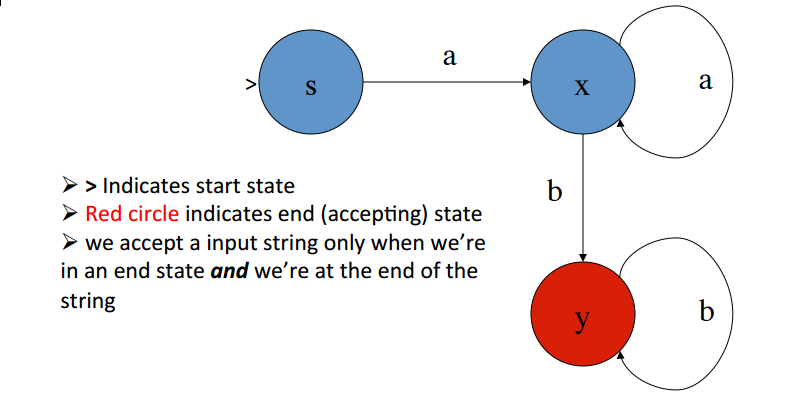
\includegraphics[width=10cm]{aplusbplus.png}}

  $L = \{a^+b^+\}$


\end{frame}

\begin{frame}[fragile]{What is a FSM?}

  \only<1>{\centerline{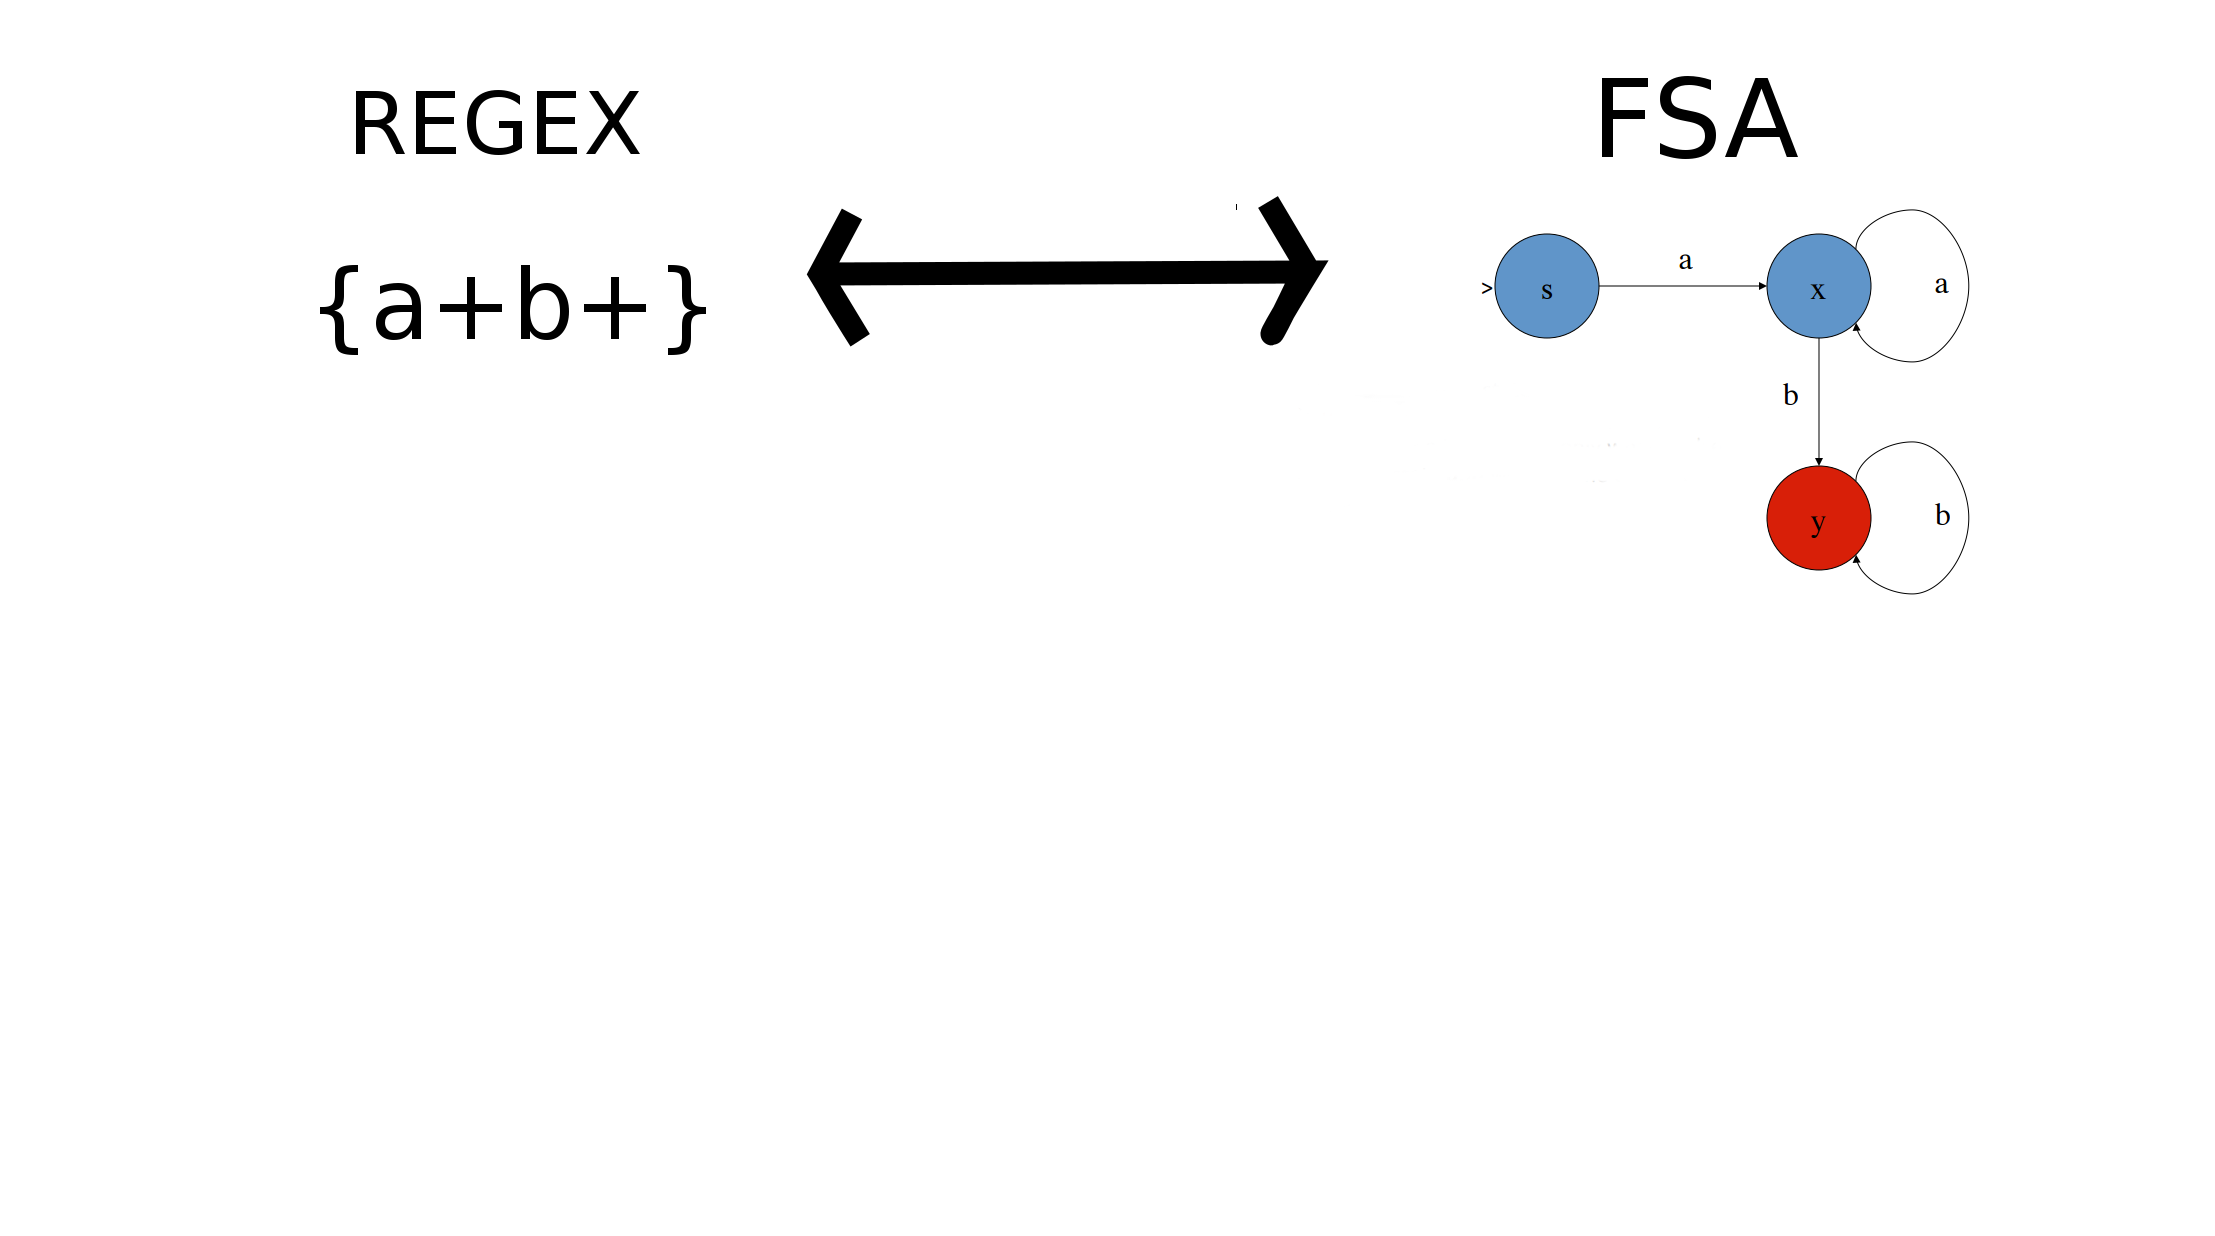
\includegraphics[width=10cm]{fsare.png}}}
  \only<2>{\centerline{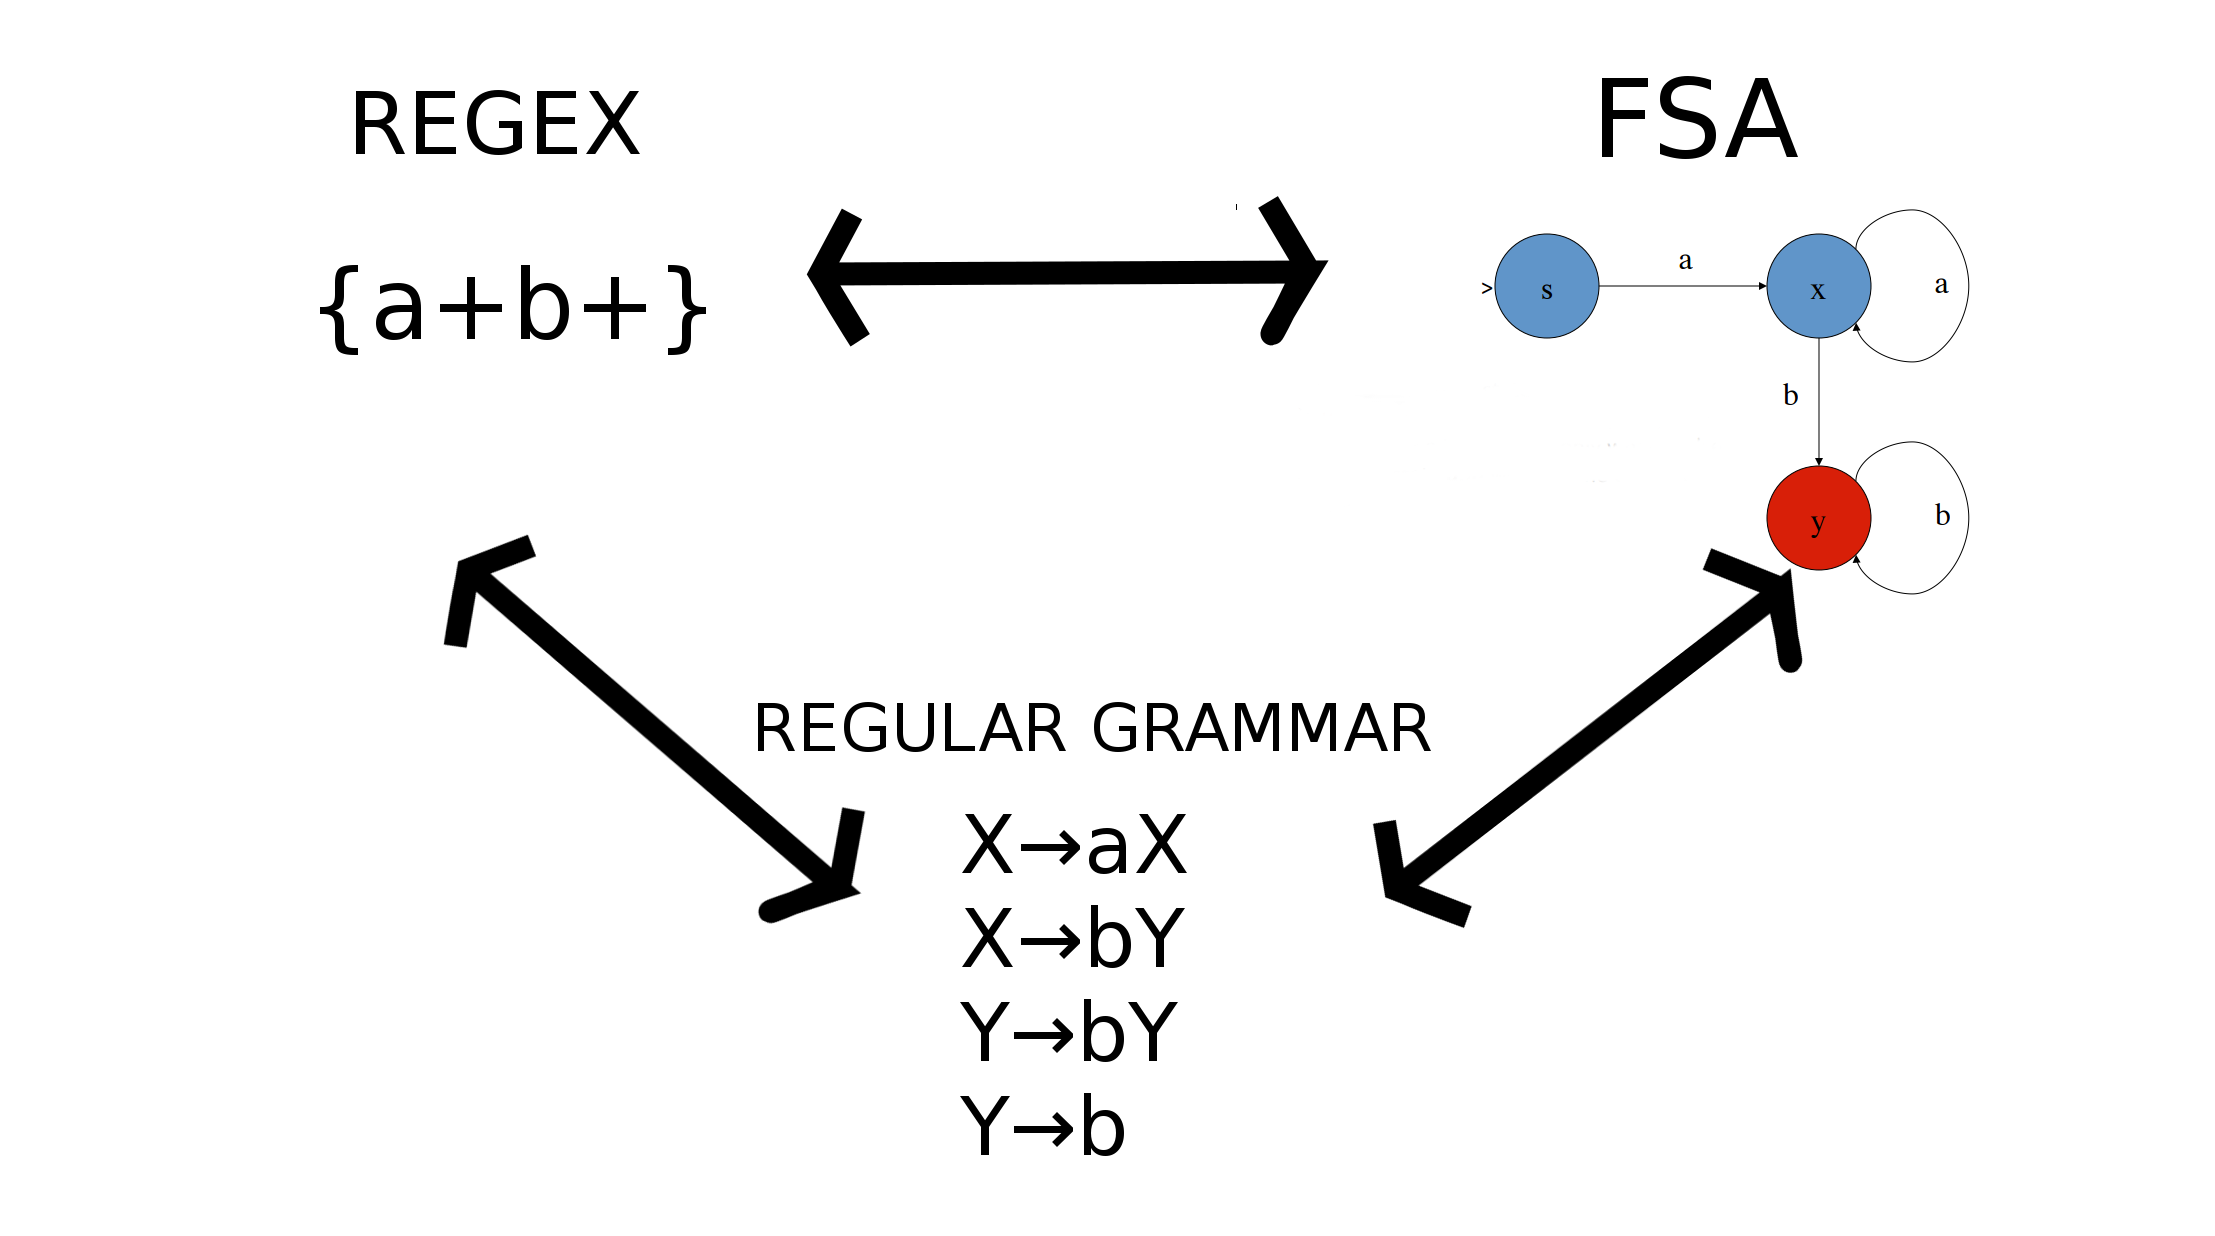
\includegraphics[width=10cm]{fsarerg.png}}}
  \only<3>{\centerline{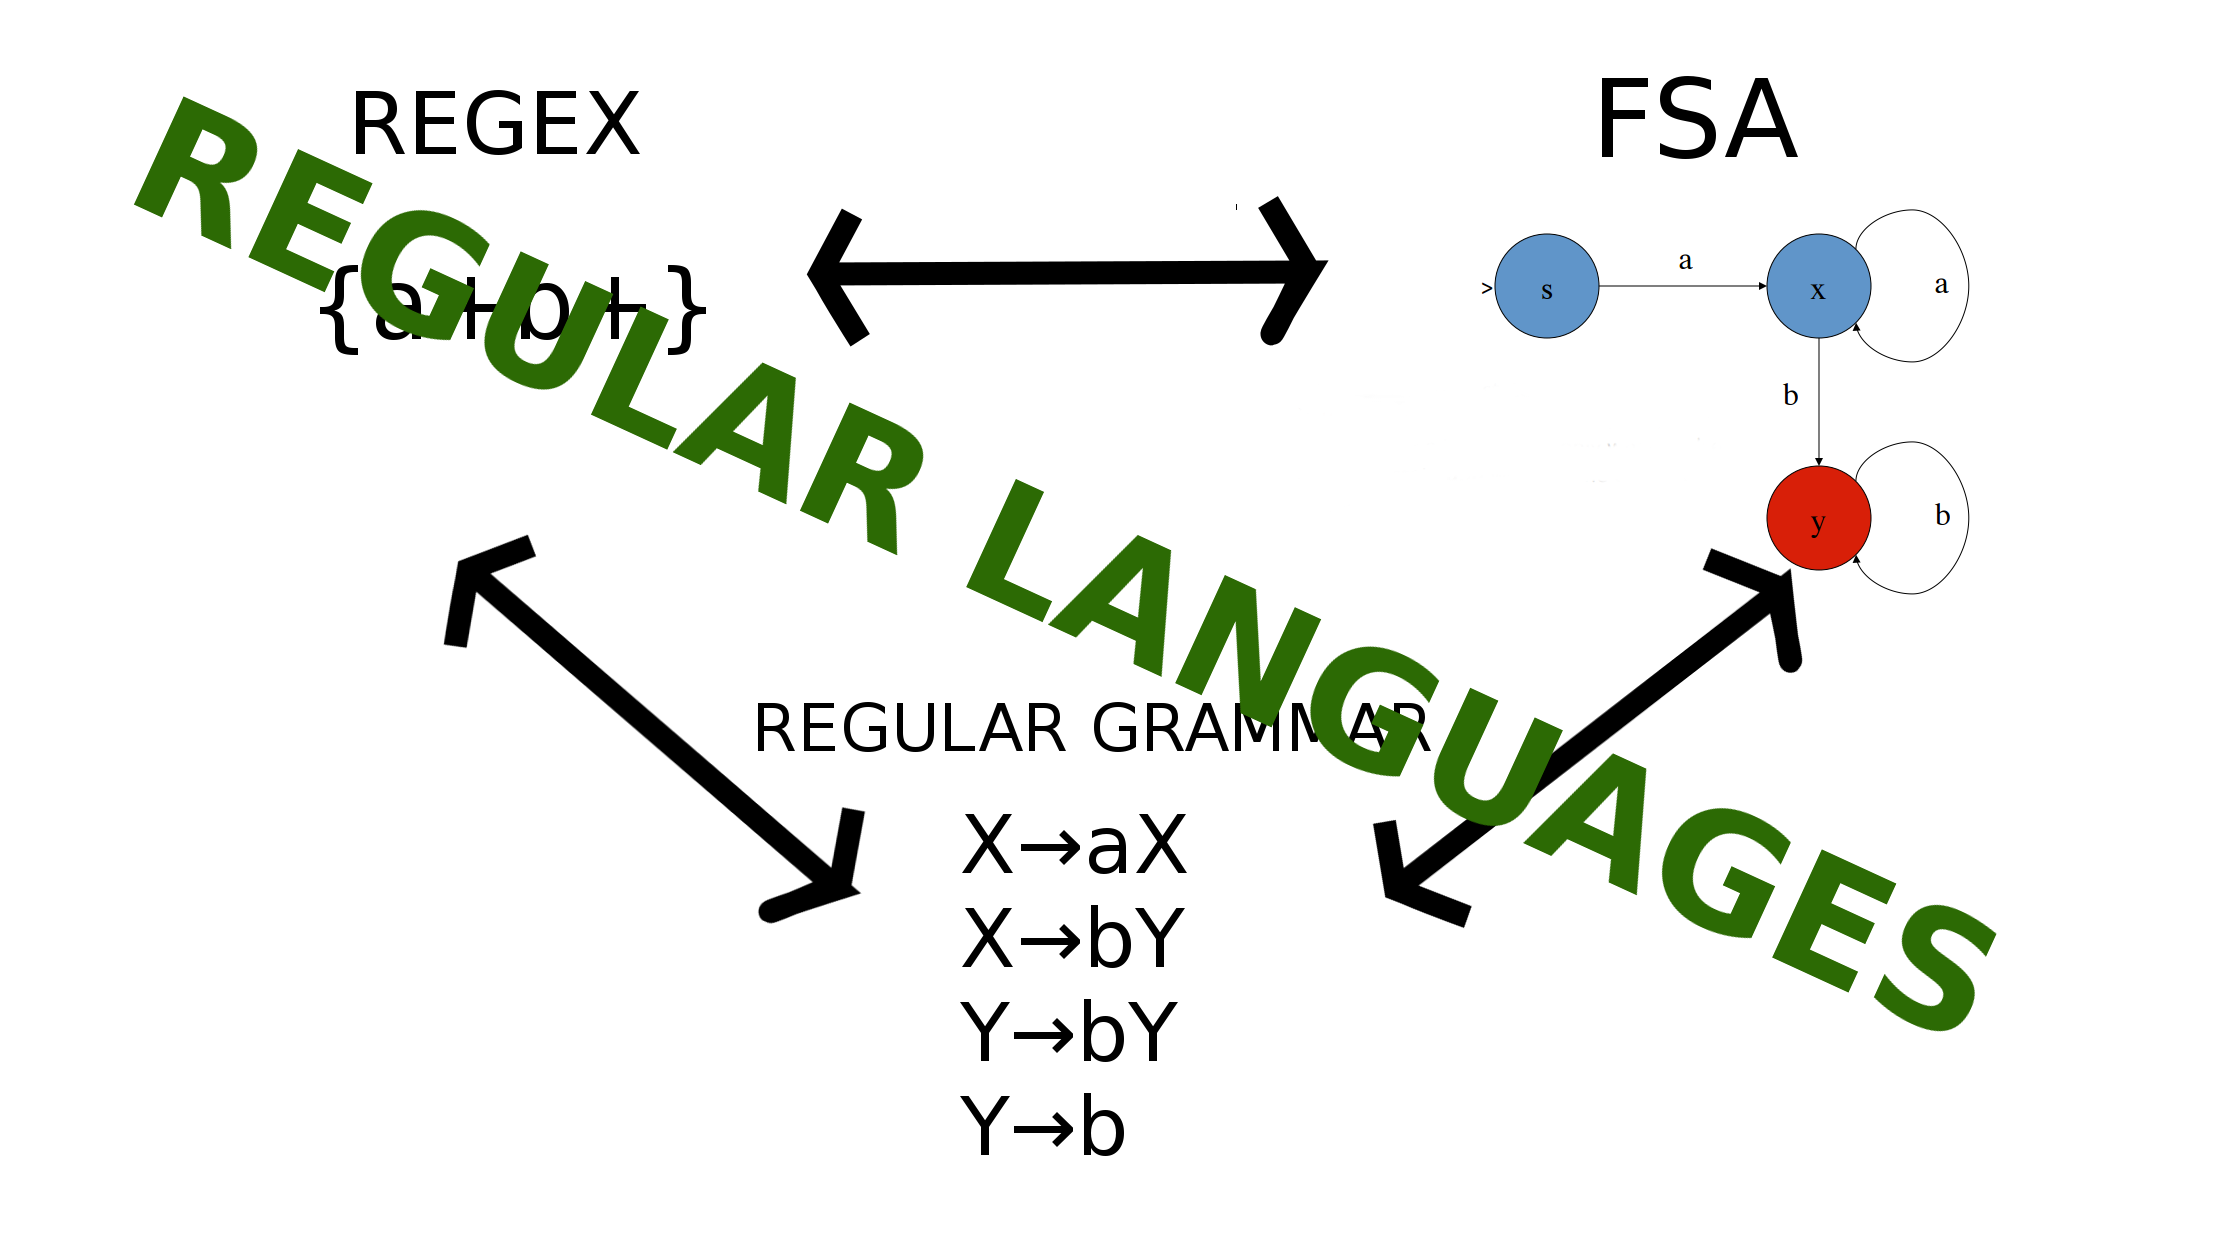
\includegraphics[width=10cm]{reglang.png}}}


\end{frame}


\begin{frame}[fragile]{Chomsky Hierarchy}

  \only<1>{\centerline{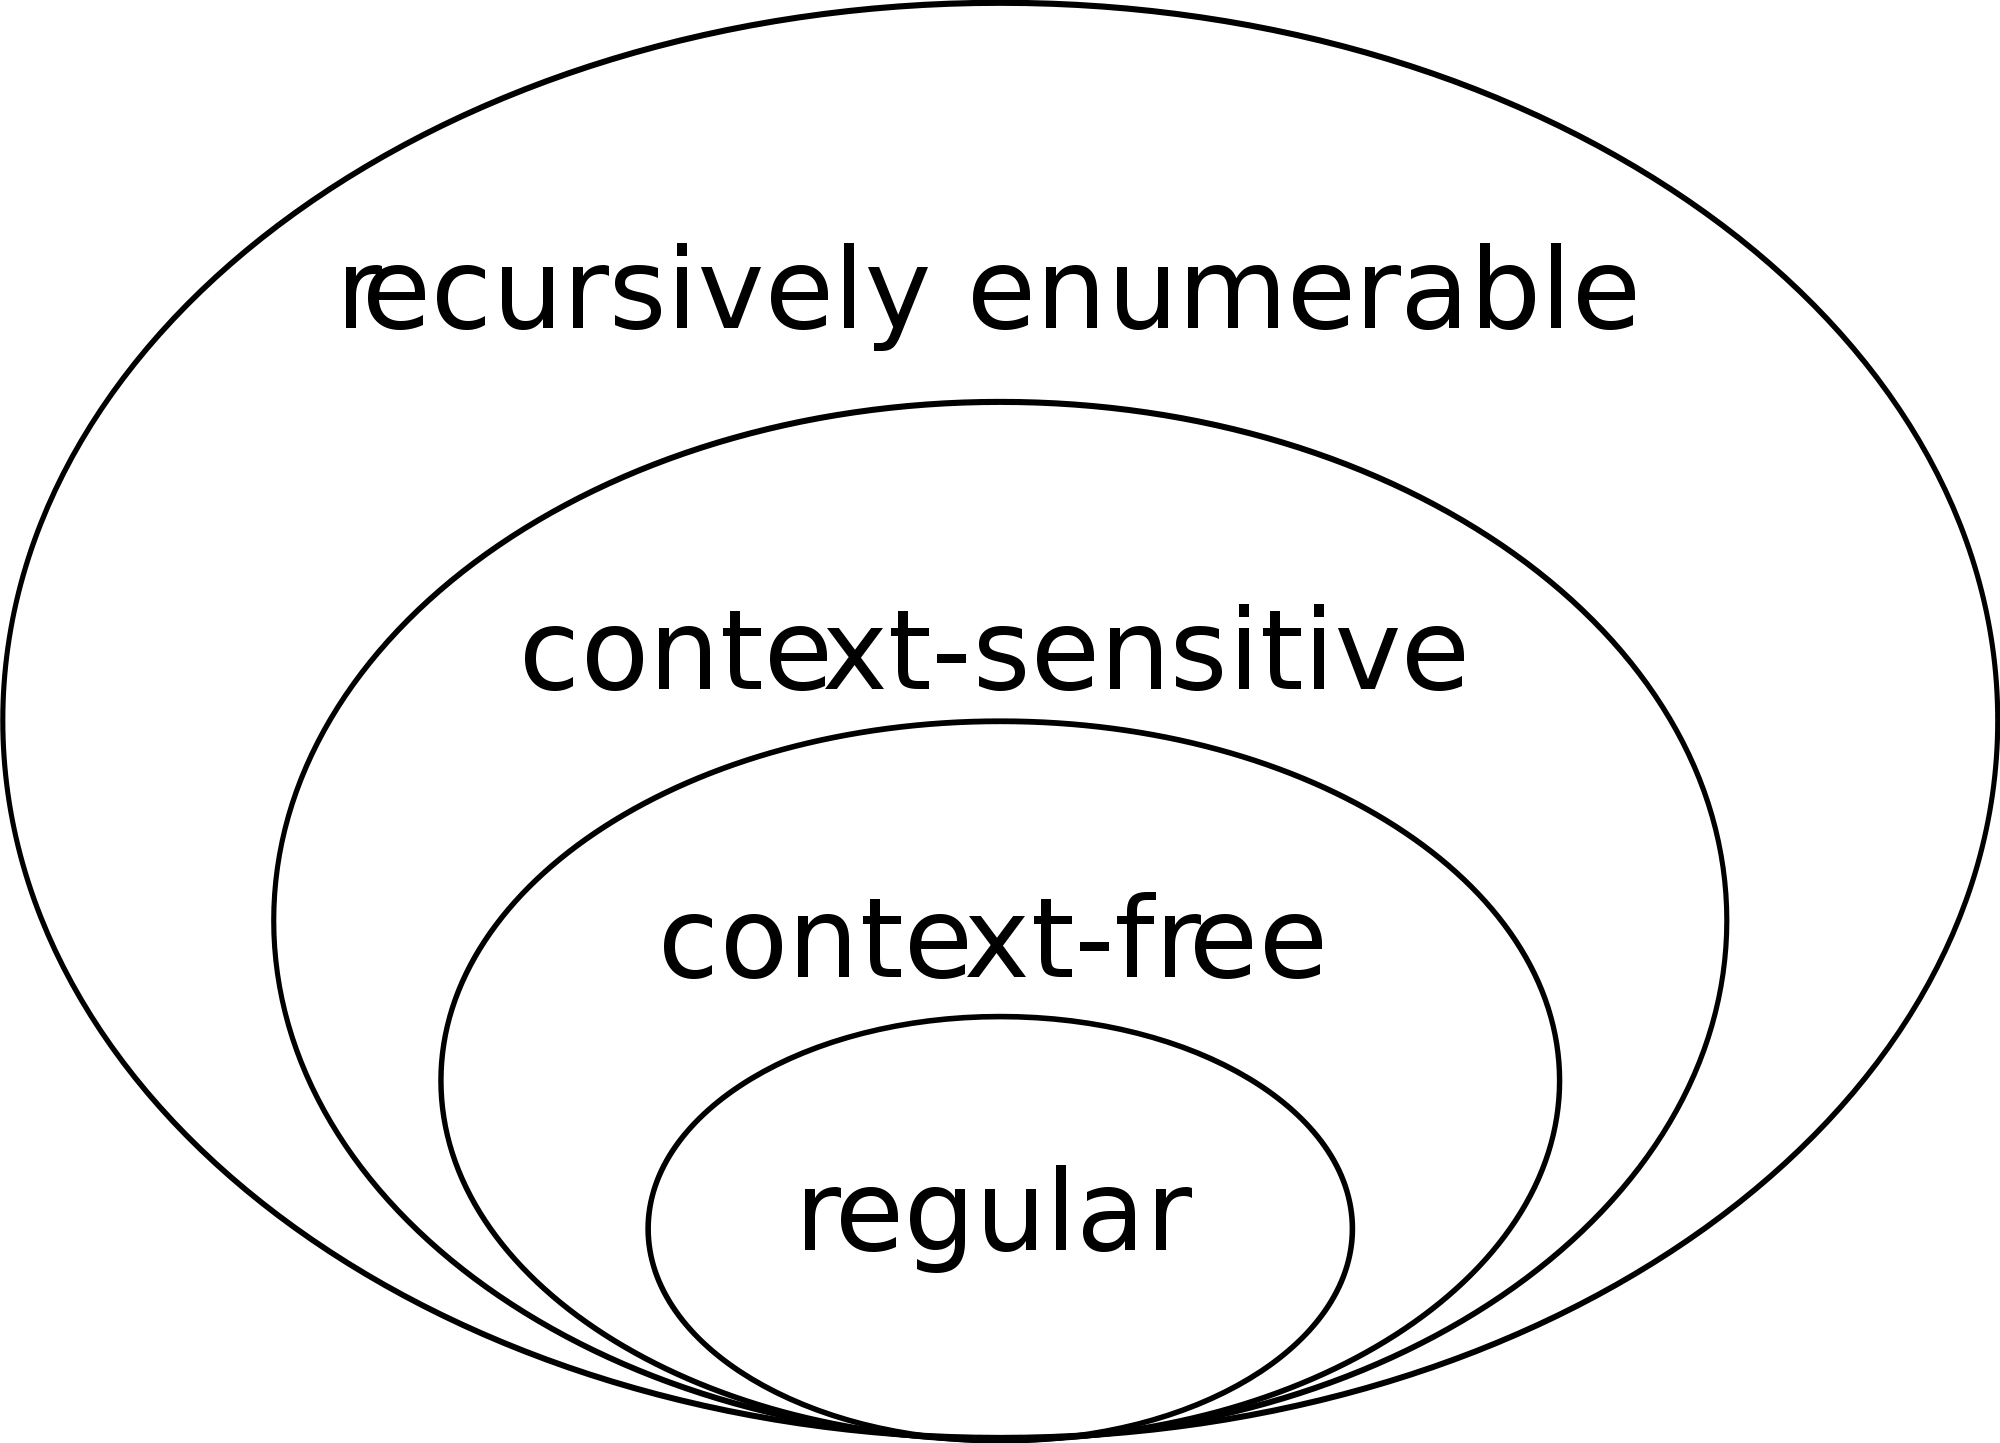
\includegraphics[width=10cm]{2000px-Chomsky-hierarchy.svg.png}}}
  \only<2>{\centerline{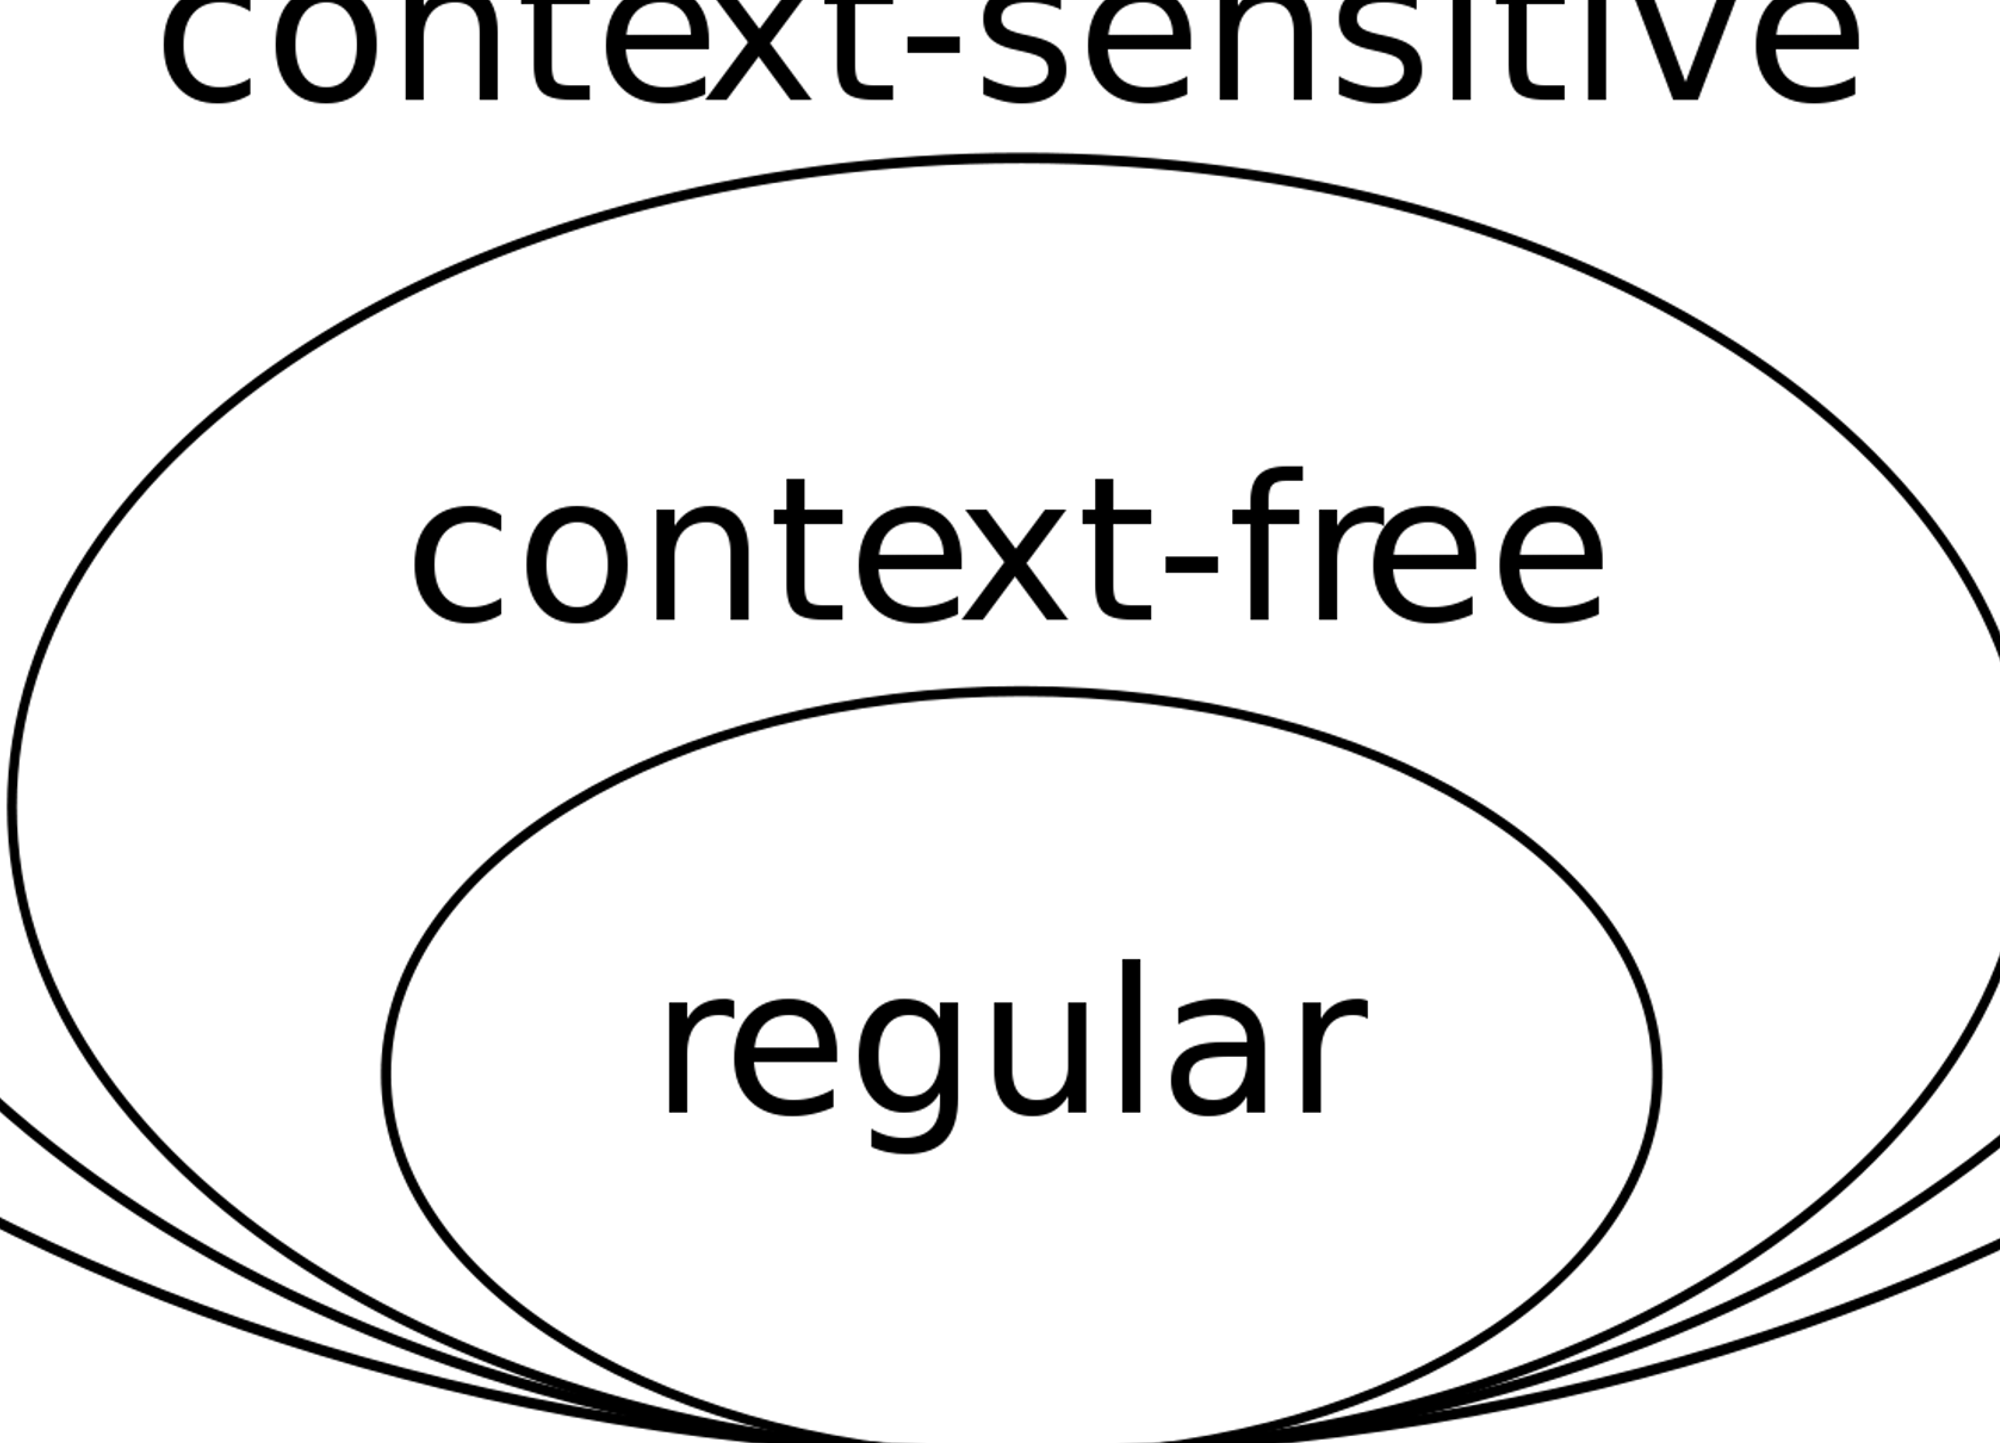
\includegraphics[width=10cm]{hierarchyzoomed.png}}}
  \only<3>{\centerline{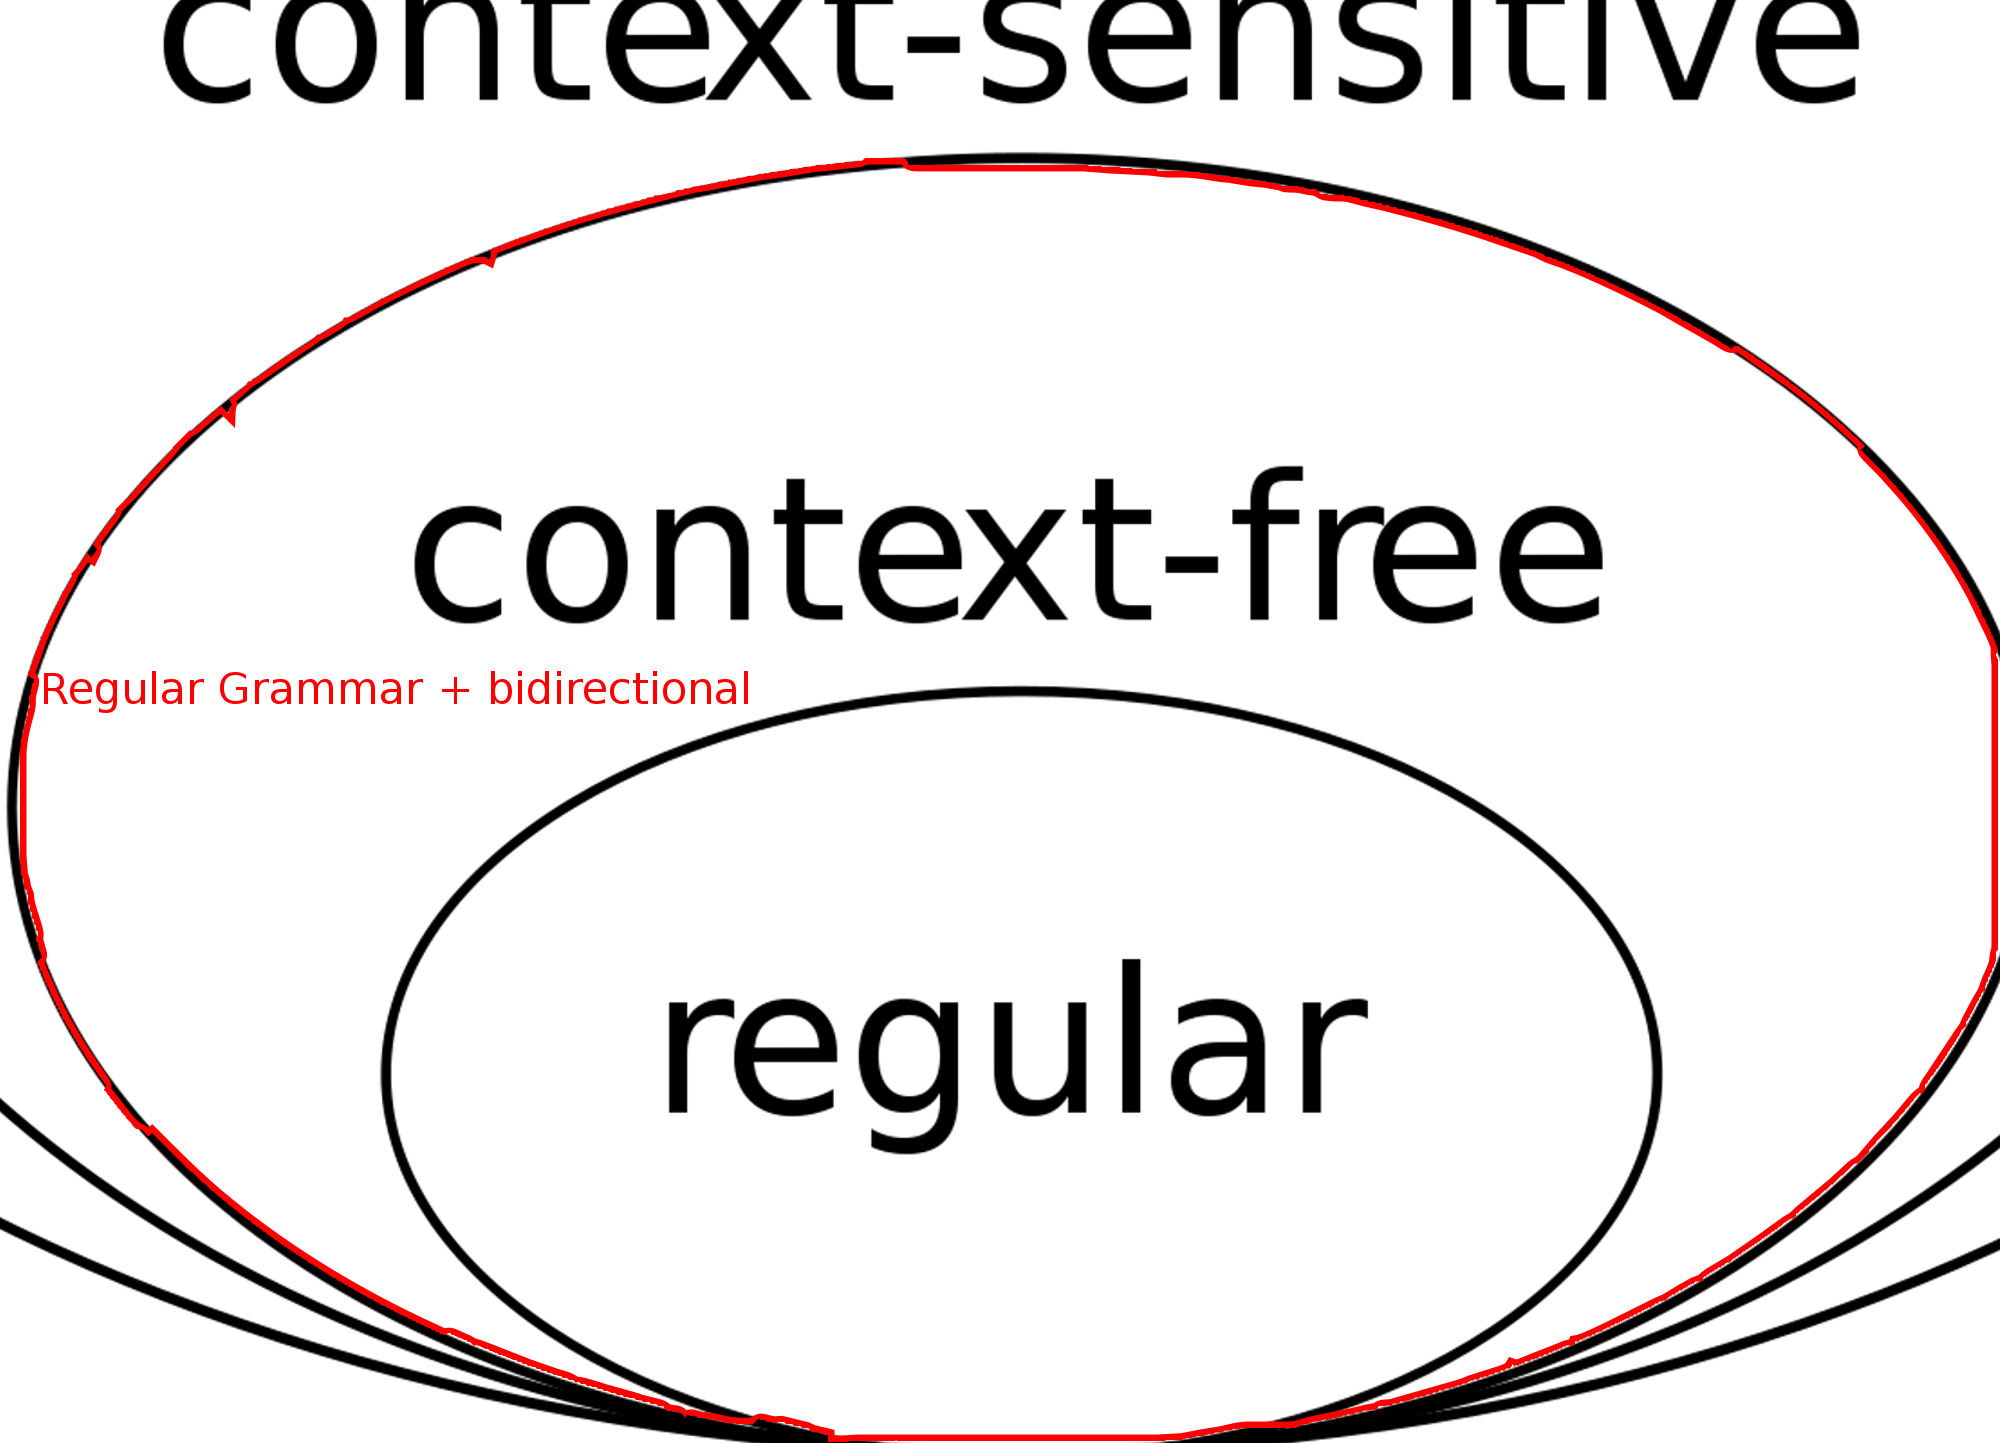
\includegraphics[width=10cm]{bidirectionalgrammar.png}}}
  \only<4>{\centerline{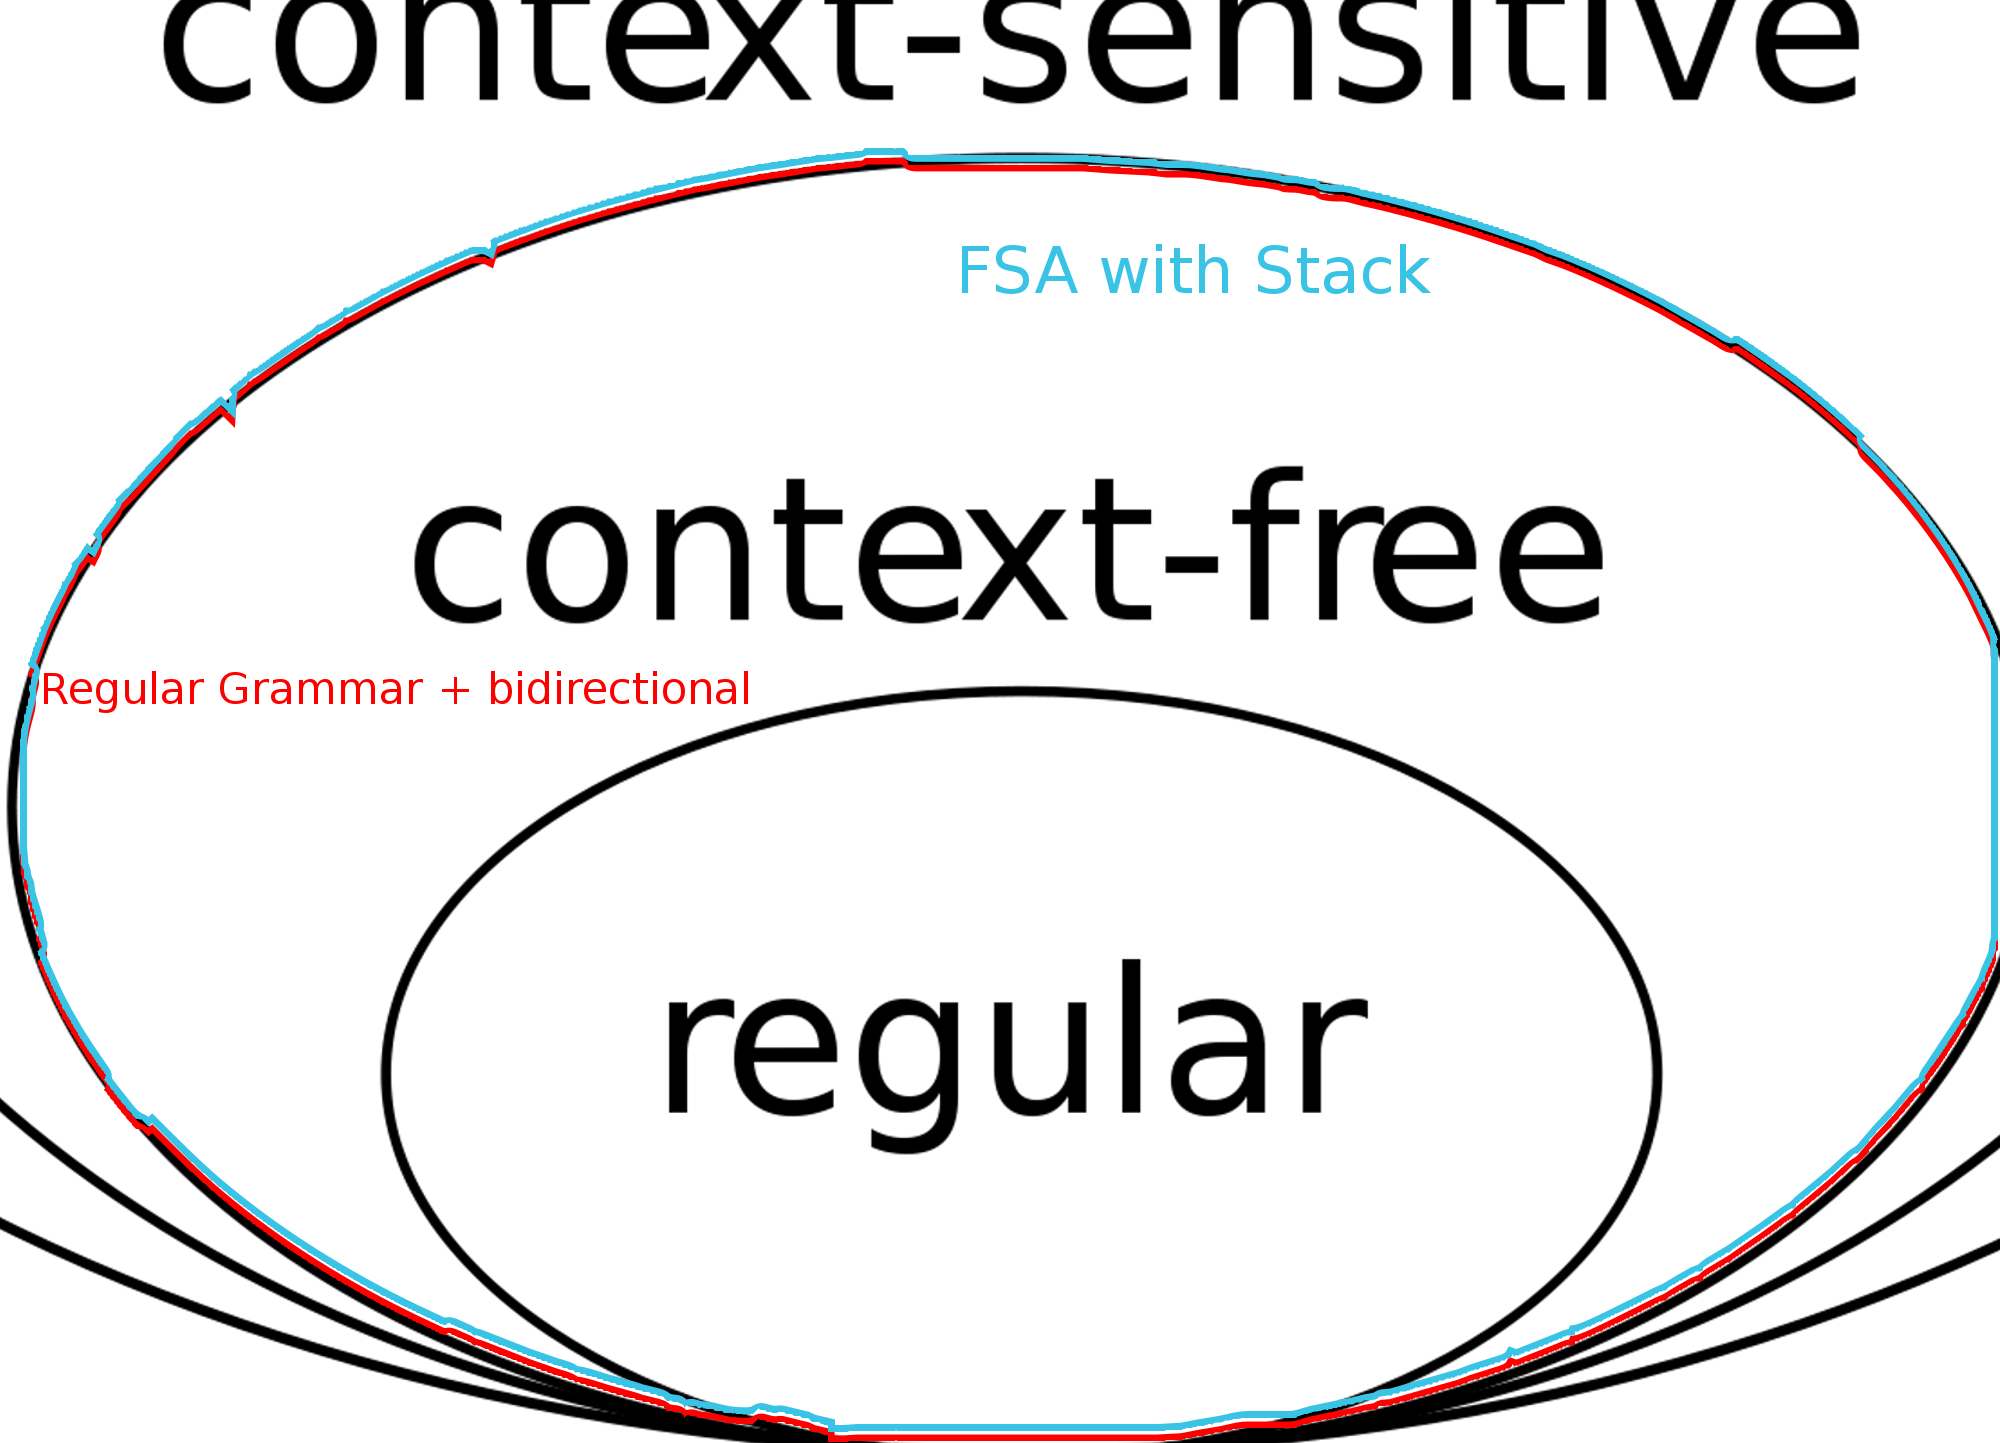
\includegraphics[width=10cm]{fsastack.png}}}
  \only<5>{\centerline{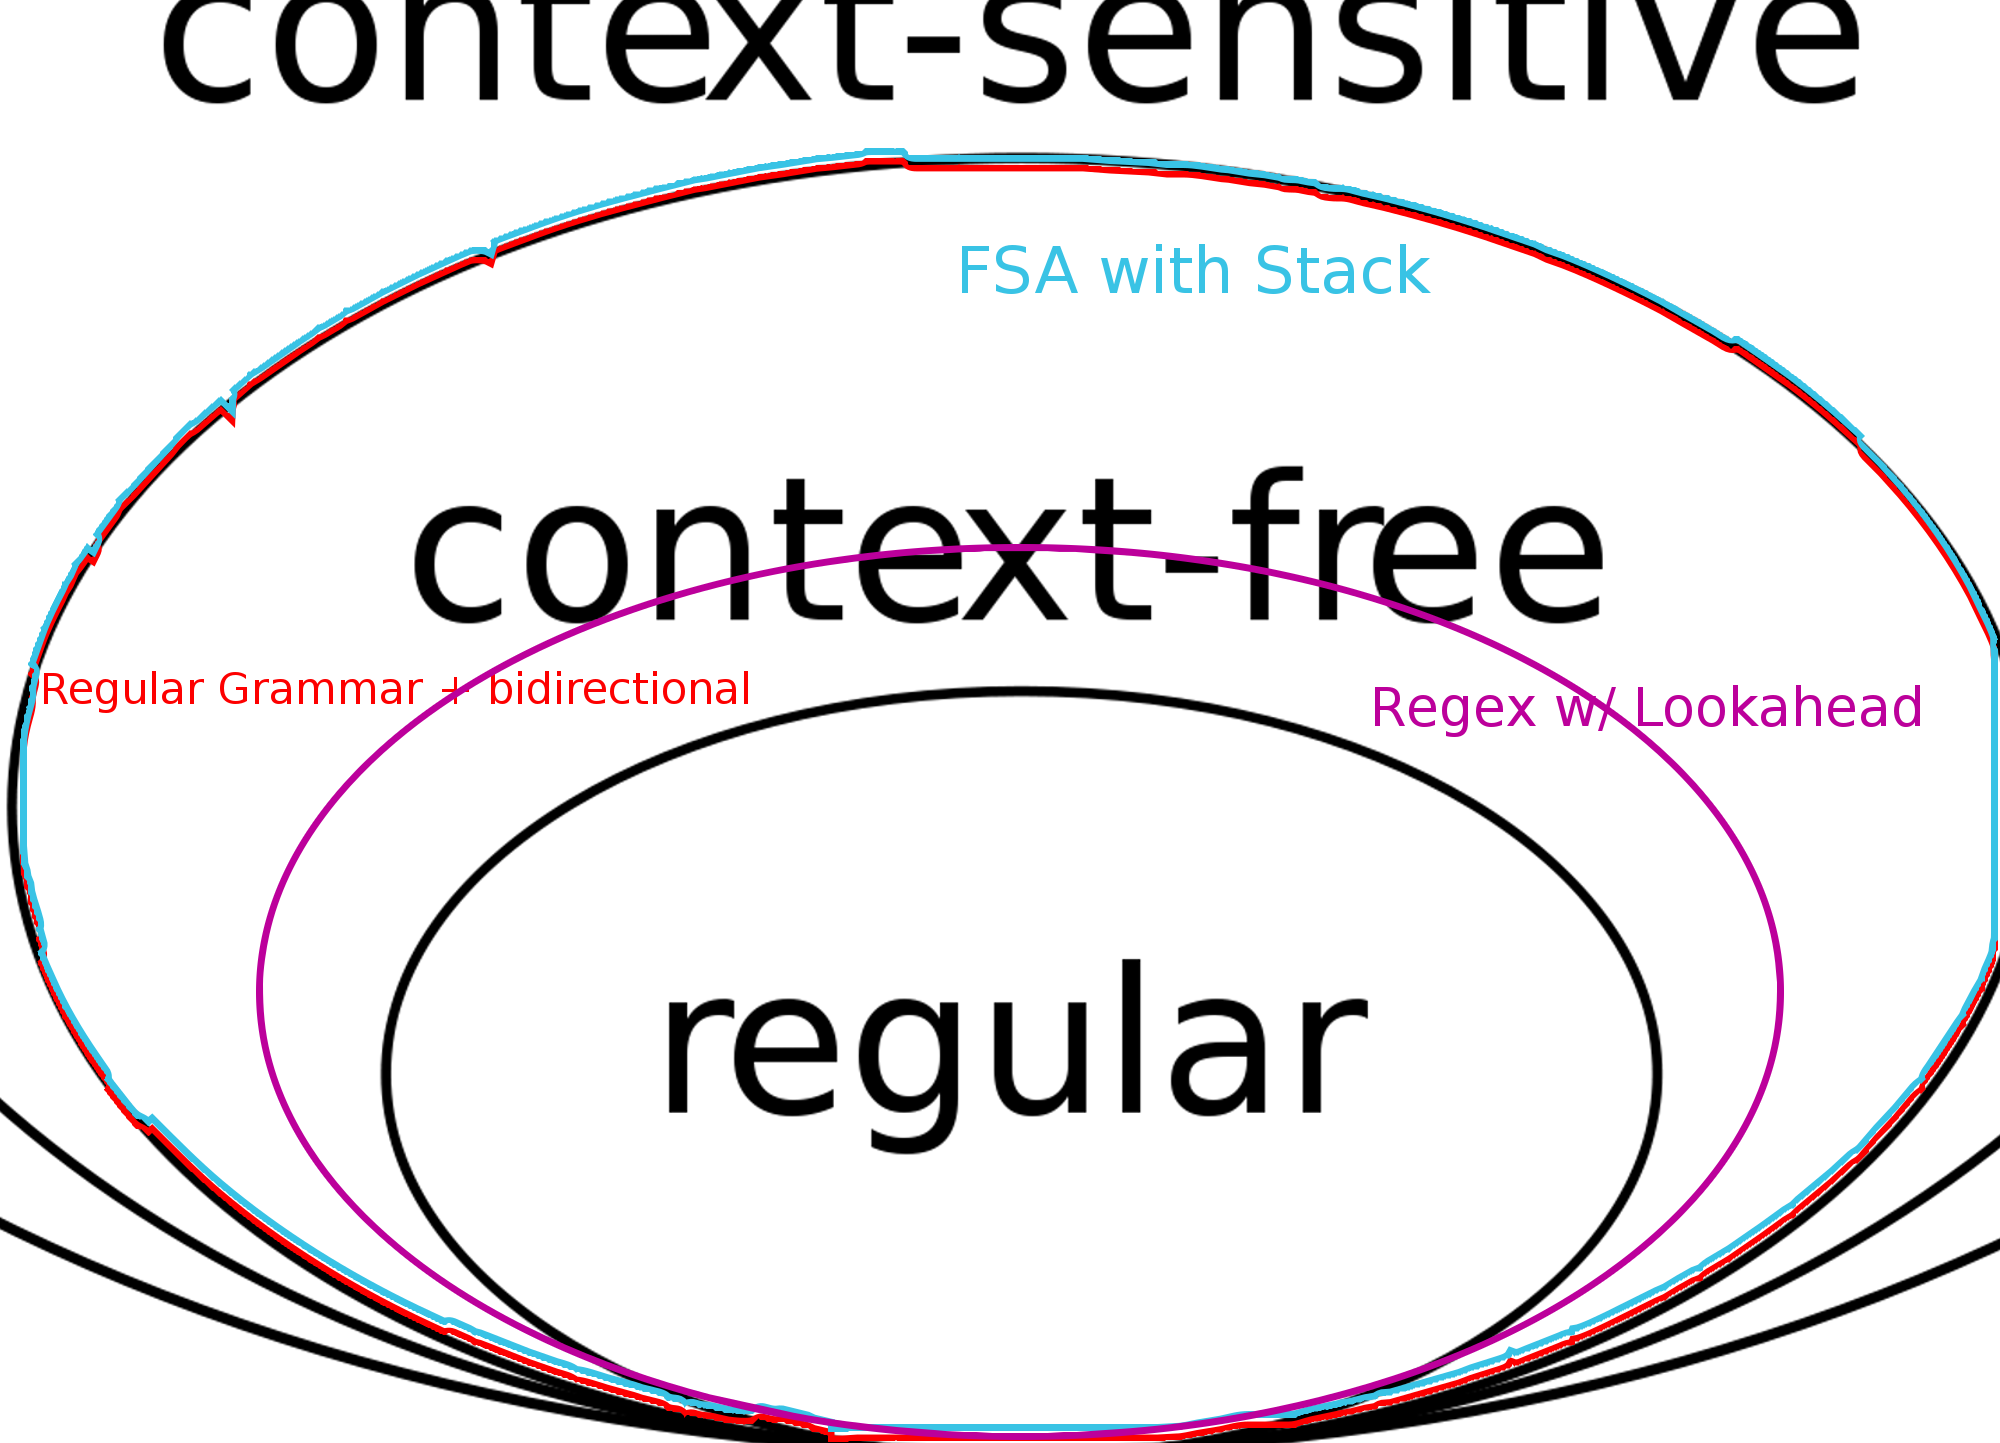
\includegraphics[width=10cm]{regexlookahead.png}}}
  \only<6>{\centerline{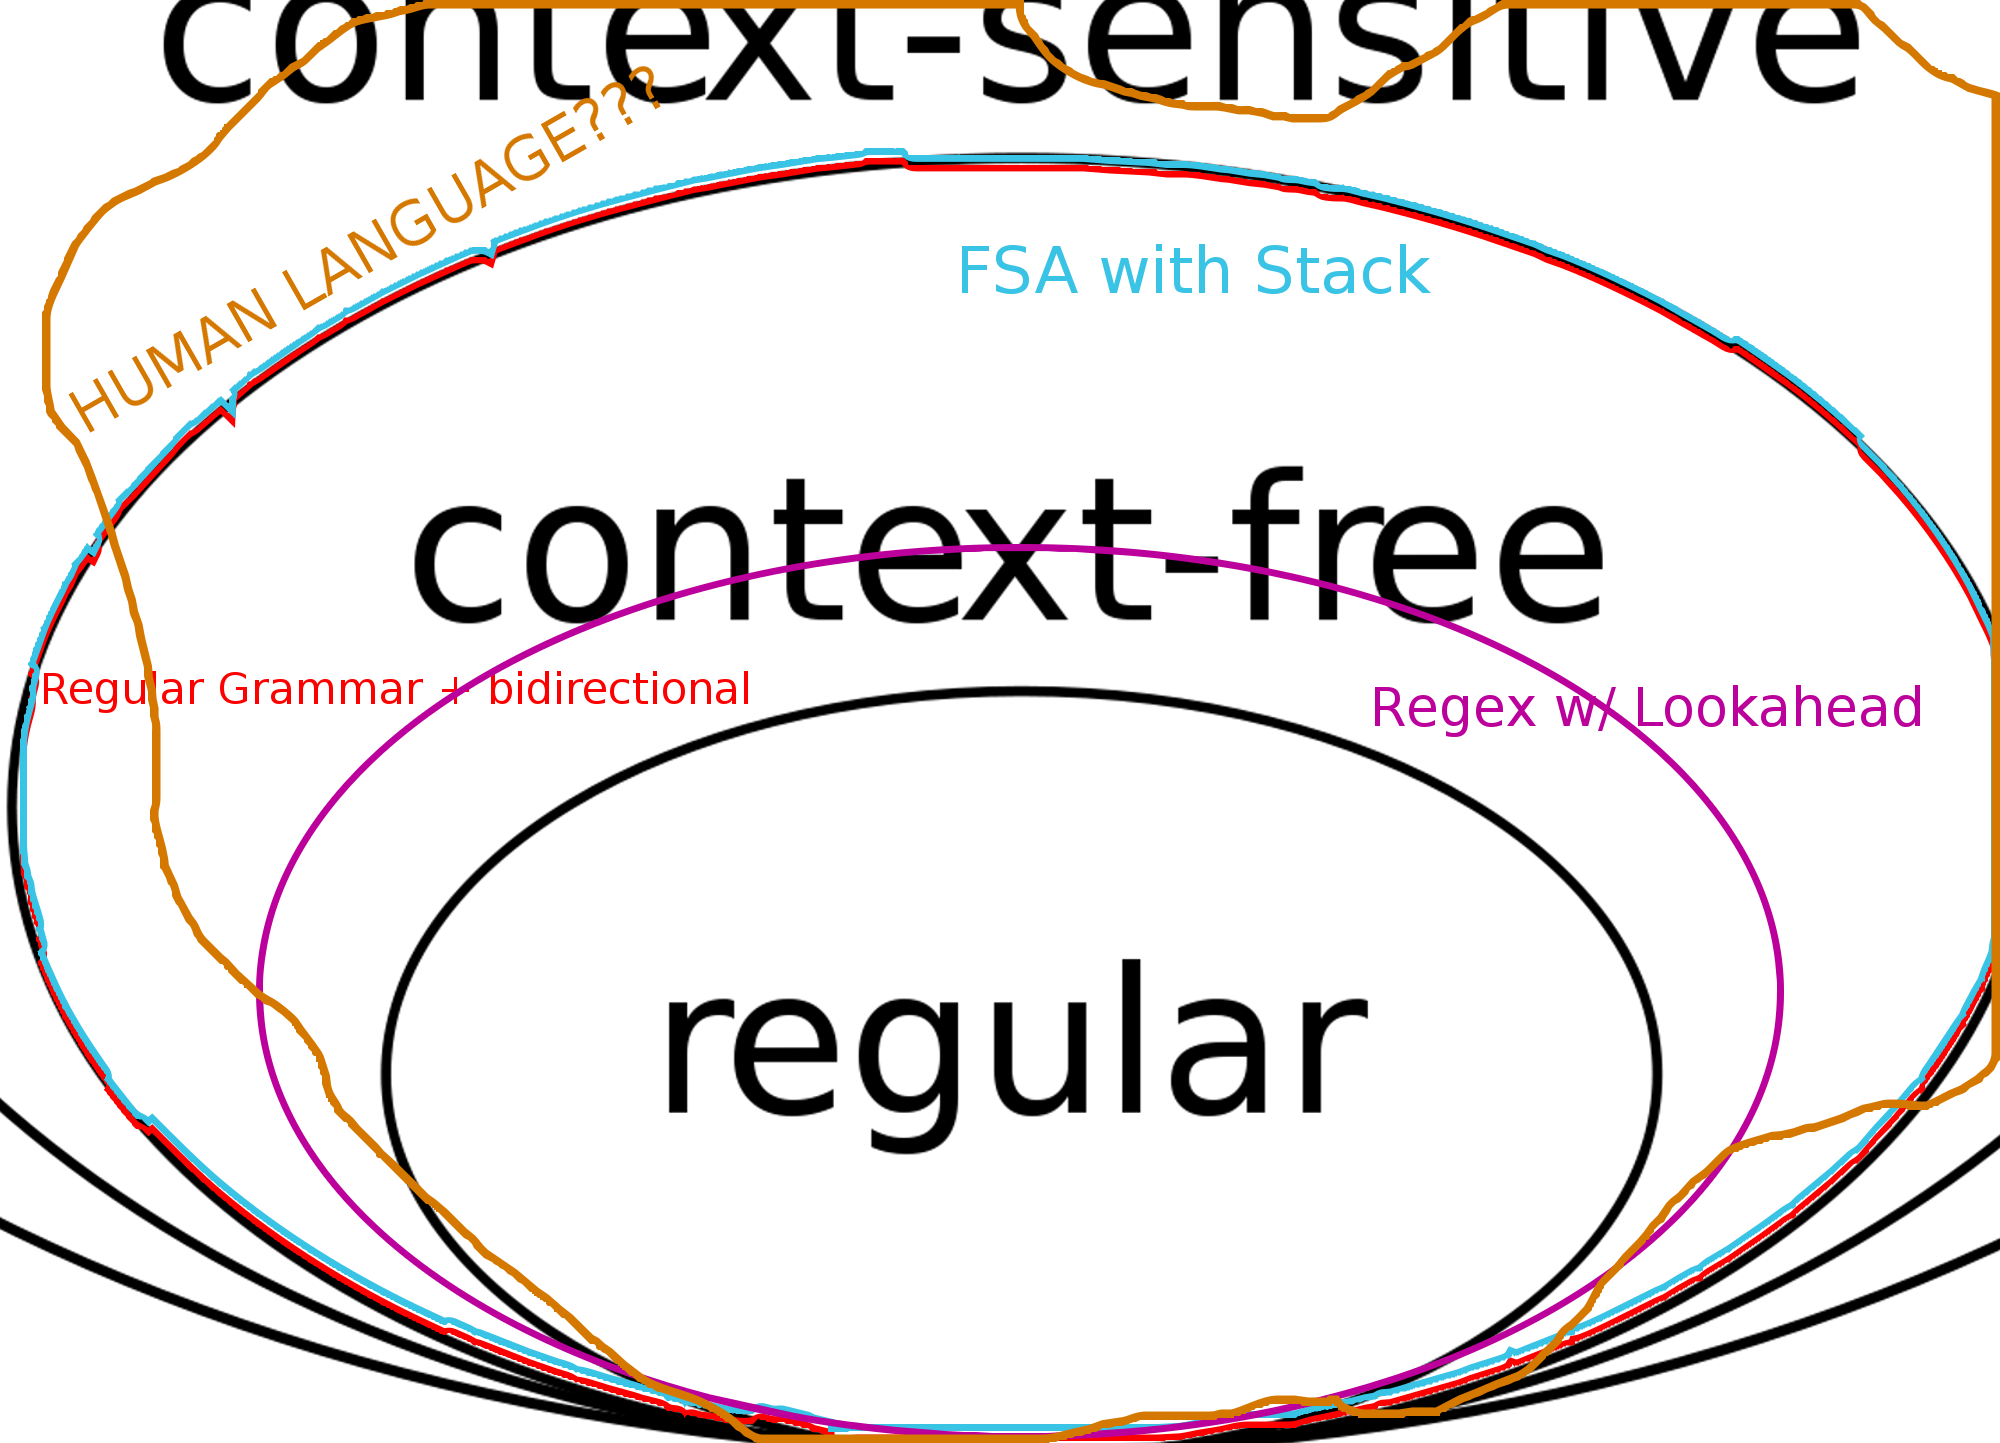
\includegraphics[width=10cm]{humanlanguage.png}}}
  \only<7>{\centerline{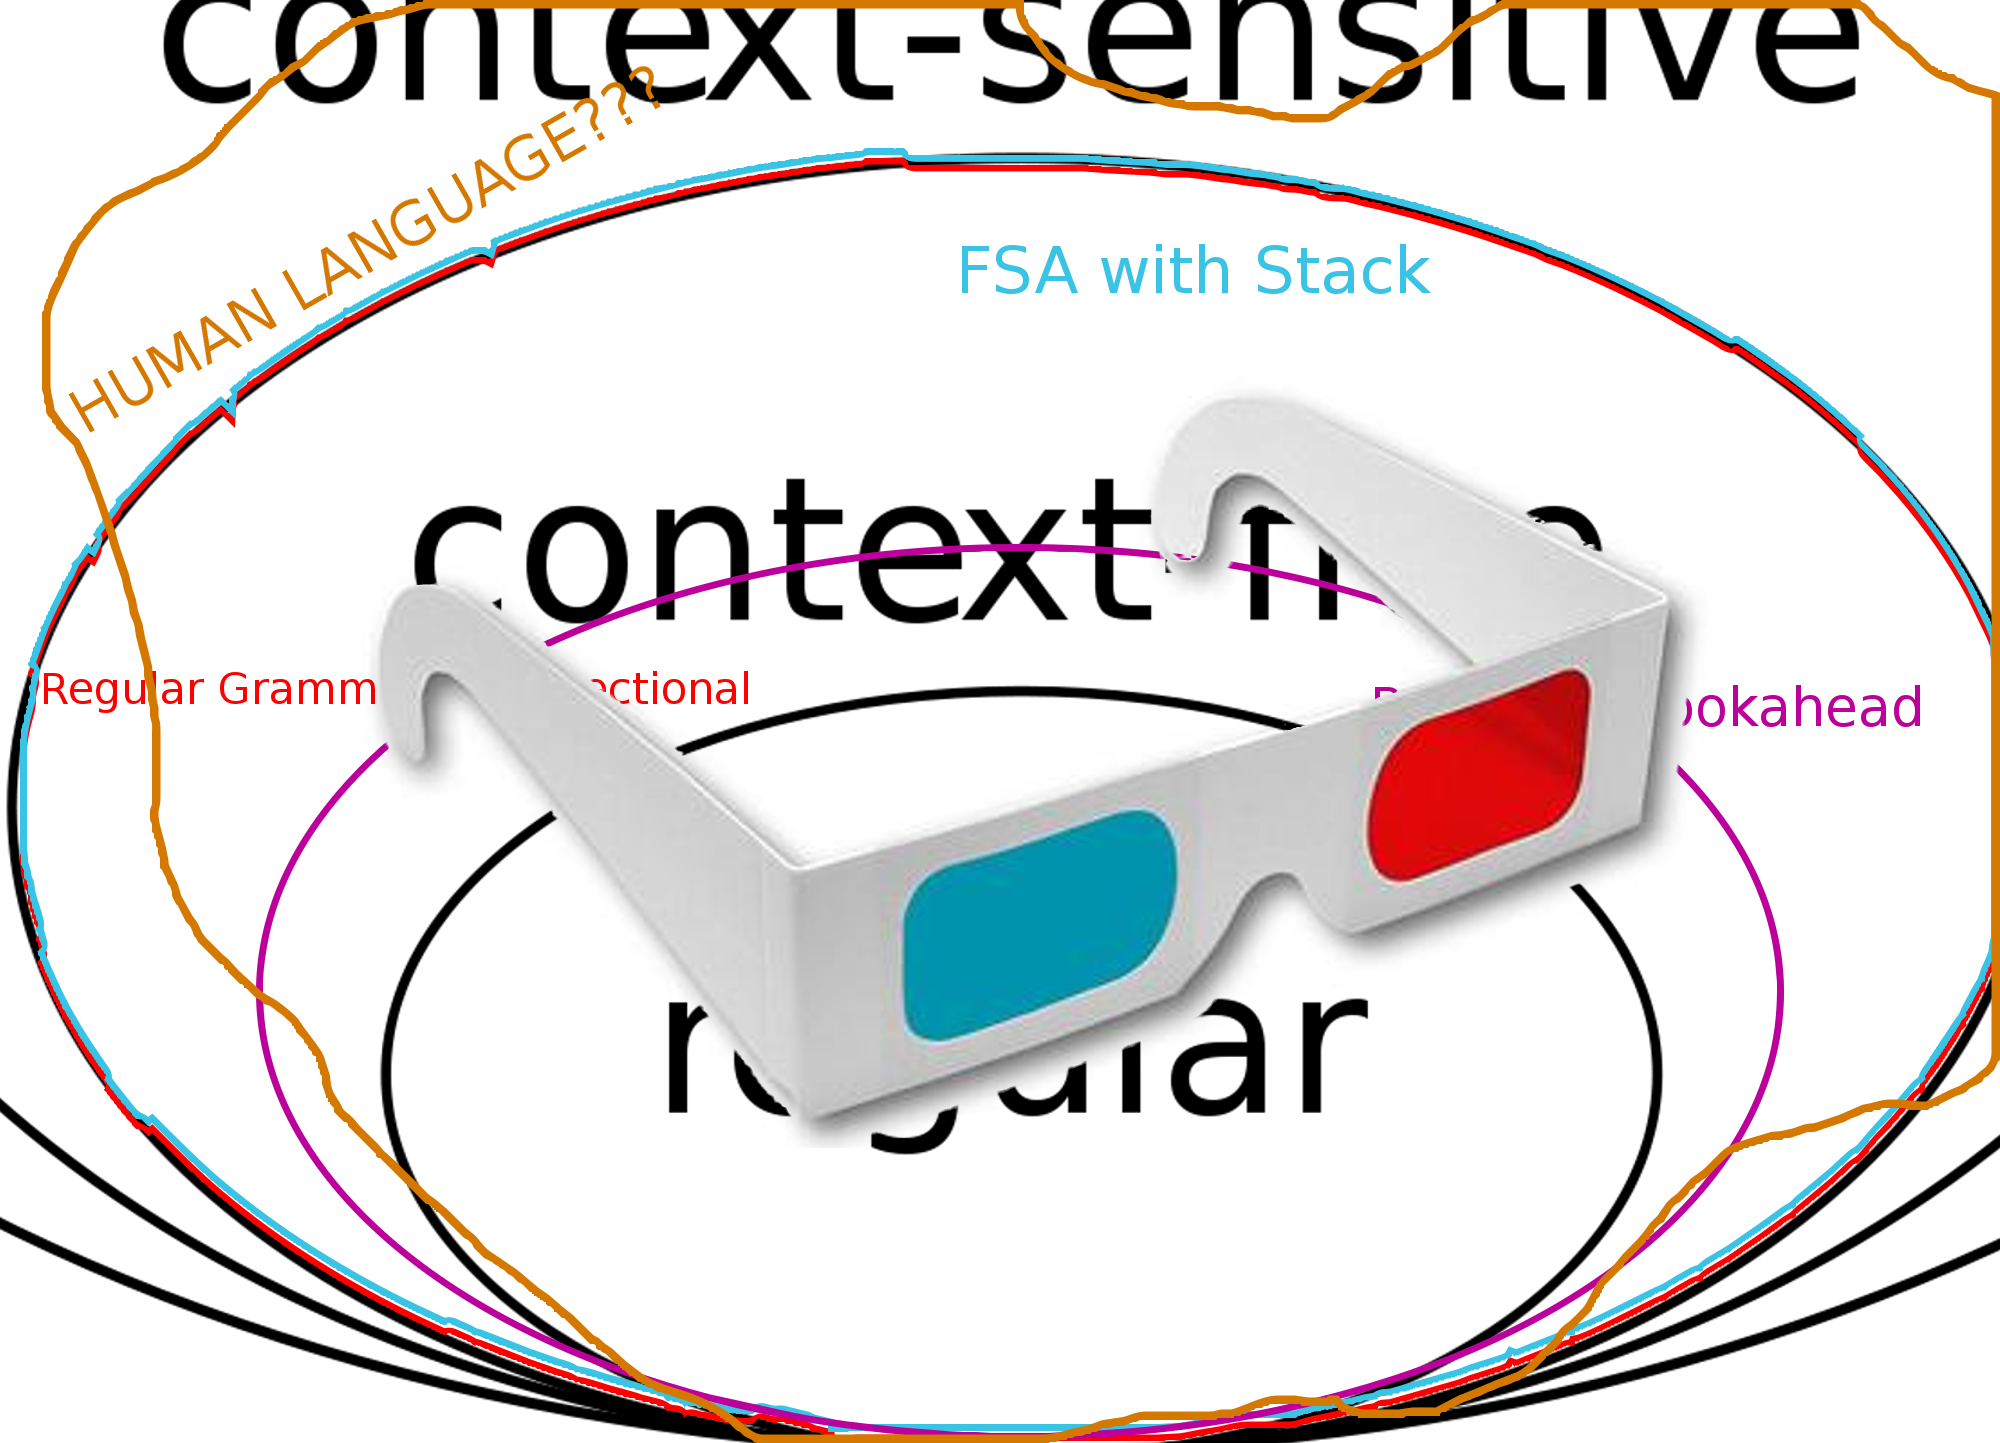
\includegraphics[width=10cm]{3djoke.png}}}



\end{frame}

\begin{frame}[fragile]{FST}

A finite state machine that turns one regular language into another regular language. 

\pause

\begin{figure}
\centering
\begin{subfigure}
\centering
  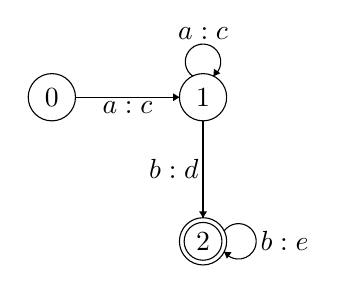
\begin{tikzpicture}[scale=.1]
  \tikzstyle{every node}+=[inner sep=0pt]
  \draw [black] (20.7,-25.1) circle (3);
  \draw (20.7,-25.1) node {$0$};
  \draw [black] (39.9,-25.1) circle (3);
  \draw (39.9,-25.1) node {$1$};
  \draw [black] (39.9,-43.4) circle (3);
  \draw (39.9,-43.4) node {$2$};
  \draw [black] (39.9,-43.4) circle (2.4);
  \draw [black] (23.7,-25.1) -- (36.9,-25.1);
  \fill [black] (36.9,-25.1) -- (36.1,-24.6) -- (36.1,-25.6);
  \draw (30.3,-25.6) node [below] {$a:c$};
  \draw [black] (38.577,-22.42) arc (234:-54:2.25);
  \draw (39.9,-17.85) node [above] {$a:c$};
  \fill [black] (41.22,-22.42) -- (42.1,-22.07) -- (41.29,-21.48);
  \draw [black] (39.9,-28.1) -- (39.9,-40.4);
  \fill [black] (39.9,-40.4) -- (40.4,-39.6) -- (39.4,-39.6);
  \draw (39.4,-34.25) node [left] {$b:d$};
  \draw [black] (42.58,-42.077) arc (144:-144:2.25);
  \draw (47.15,-43.4) node [right] {$b:e$};
  \fill [black] (42.58,-44.72) -- (42.93,-45.6) -- (43.52,-44.79);
  \end{tikzpicture}
\end{subfigure}
\pause
\begin{subfigure}
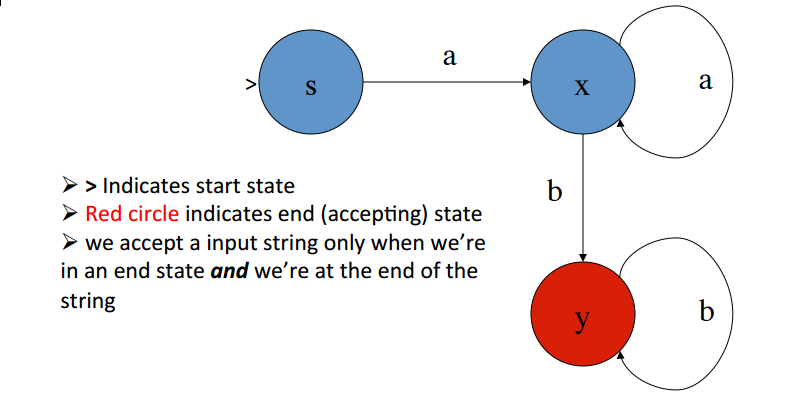
\includegraphics[width=5cm]{aplusbplus.png}

\end{subfigure}
\end{figure}
\pause

FST that transforms $\{a+b+\}$ to $\{c+de*\}$


\end{frame}

\begin{frame}[fragile]{Formal Definition}

  \pause

  $\langle \Sigma, S, s_0, \delta, F \rangle$


  \begin{description}

    \item[\Sigma] alphabet
    \item[$S$] states
    \item[$s_0 \in S$] start state
    \item[\delta] transition function 

    $\delta: S,\Sigma \to S$

      (Can be partial or total)
    \item[F \subset S] final states 

    (can be \emptyset) 

  \end{description}




\end{frame}

\section{Uses in Computational Linguistics}

\begin{frame}[fragile]{Morphology!}

  There are dictionaries of derived forms of words, but these can never be fully complete. 

  Cortois and Laporte (1991) demonstrated that most terms found missing from LADL\footnote{Labratorie d'Automatique Documentaire et Linguistique}s DELAS\footnote{Dictionairie Electronique du LADL S} by comparing against natural language text are derived forms that were missed. 




\end{frame}


\begin{frame}[fragile]{SDICOS, the morphological transducer}

  Problem:

  \begin{columns}[T,onlytextwidth]
    \column{0.5\textwidth}

    \metroset{block=fill}

      \begin{block}{Present in DICOS}
        activier
      \end{block}


    \column{0.5\textwidth}

      \metroset{block=fill}

      \begin{block}{Missing from DICOS}
        activable \\
        activabilite \\
        suractivation \\
        suractivable \\

      \end{block}

  \end{columns}



  Attempts to add these to the dictionary inevitably miss many and dramatically increase the dictionary size and reduce search speed without much benefit. 






\end{frame}

\begin{frame}[fragile]{Solution: FST}
  
  Rather than storing a word list, make a transducer that changes an input word to output dictionary information. 


\end{frame}

\begin{frame}[fragile]{Solution: FST}

  \begin{itemize}
  \item inculperont $\iff$ inculper, V+f3p

  \item aimerant $\iff$ aimer, V+f3p

  \item chevaux $\iff$ cheval, N+mp

  \item carnavals $\iff$ carnaval, N+mp

  \item pommes $\iff$ pomme, N+fp

  \item pommes $\iff$ pommer, V+P2s

  \item pommes $\iff$ pommer, V+S2s

  \end{itemize}
  

  \pause

  (disambiguation problem: we don't care)

\end{frame}


\begin{frame}[fragile]
  \frametitle{SDICOF}

  \centerline{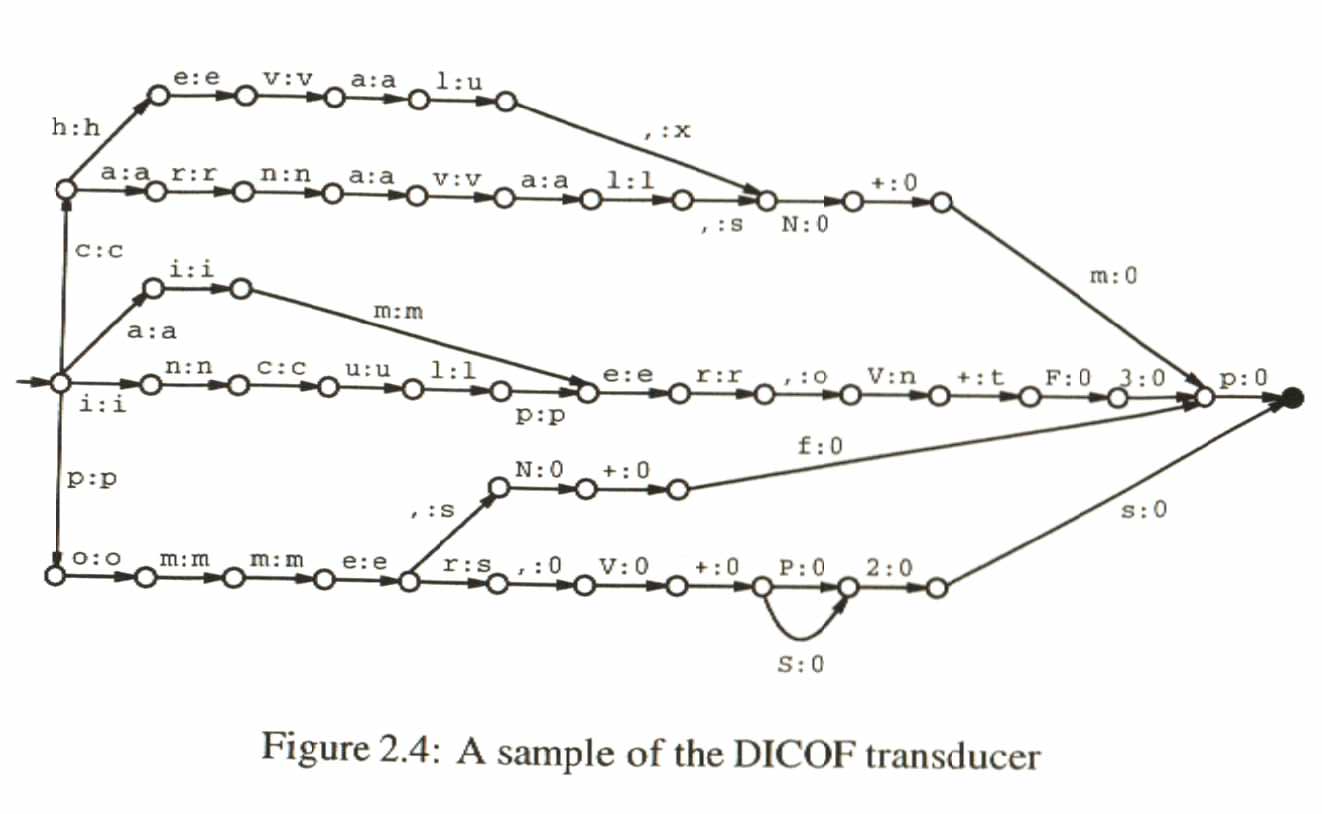
\includegraphics[width=10cm]{fig24.png}}

\end{frame}

\begin{frame}[fragile]
  \frametitle{Performance}

  \centerline{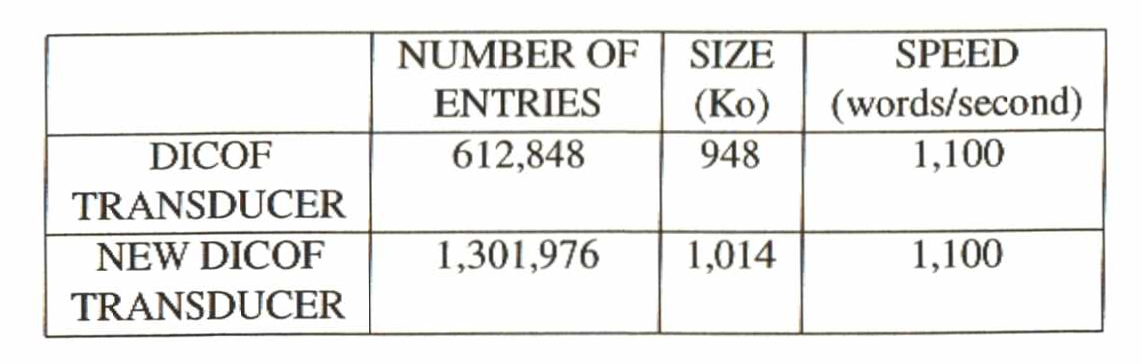
\includegraphics[width=10cm]{dicofperformance.png}}
\end{frame}

\begin{frame}[fragile]
  \frametitle{Issues}

  Not very convenient because you cannot link a derivitive in a text to the root of it's derivational tree. 

  We need a system that given a derivitive returns the trees that contain it. 
\end{frame}

\begin{frame}[fragile]
  \frametitle{New FST}

  \begin{itemize}
    \item C1 + activier + Vable.32RA/S $\iff$ coactivable
    \item I3 + C1 + activier + Vable.32RA/S $\iff$ incoactivable
    \item O1 + activier + Vable.32RA/S $\iff$ coactivable
    \item I3 + O1 + activier + Vable32RA/S $\iff$ incoactivable
  

  \end{itemize}
  \pause

  (C = symmetry of subjects, O = symmetry of objects, eg 

  ``IBM and Microsoft codeveloped OS/2'' vs ``The alarm and the lock are always coactivated'')
  
\end{frame}

\begin{frame}[fragile]
  \frametitle{SDICOS}

  \centerline{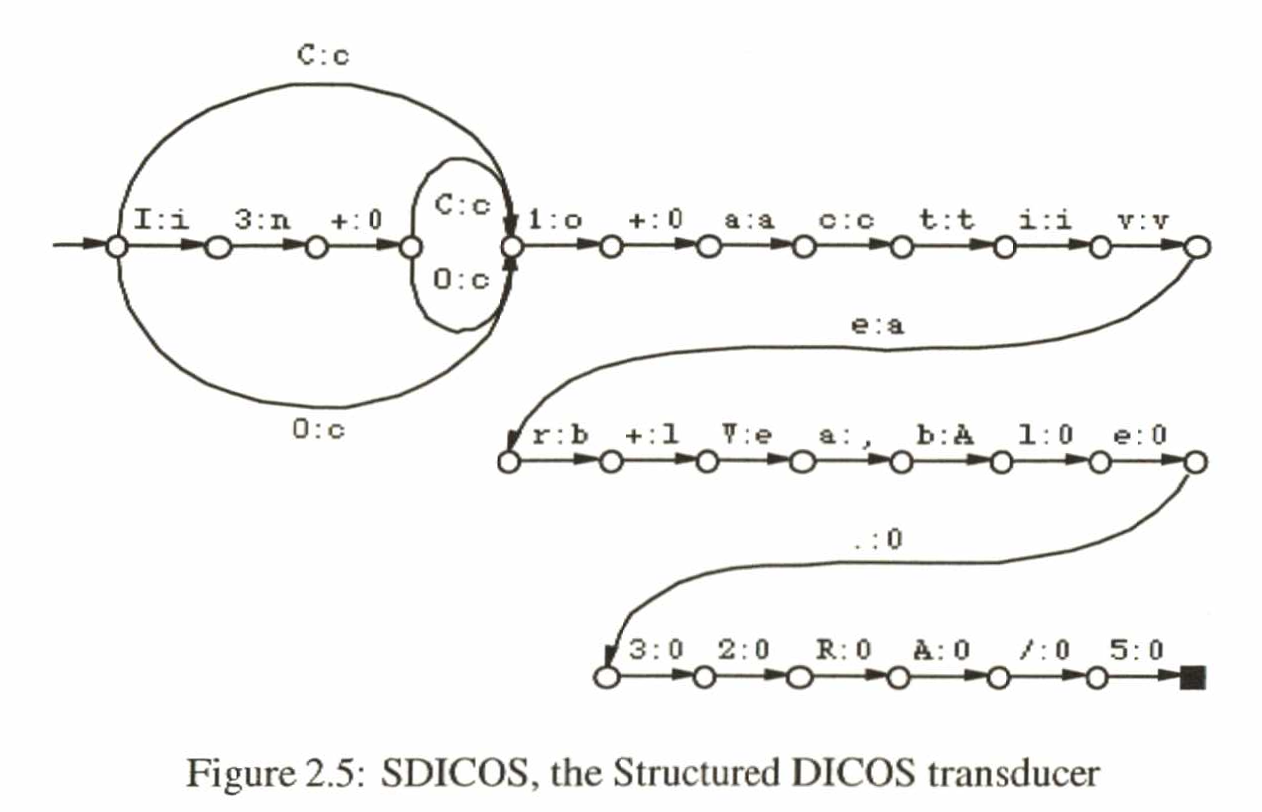
\includegraphics[width=10cm]{fig25.png}}

  \pause

  Not as fast (519 w/s), significantly smaller memory imprint (97Kb)
\end{frame}

\begin{frame}[fragile]
  \frametitle{More Generic}

  \only<1>{\centerline{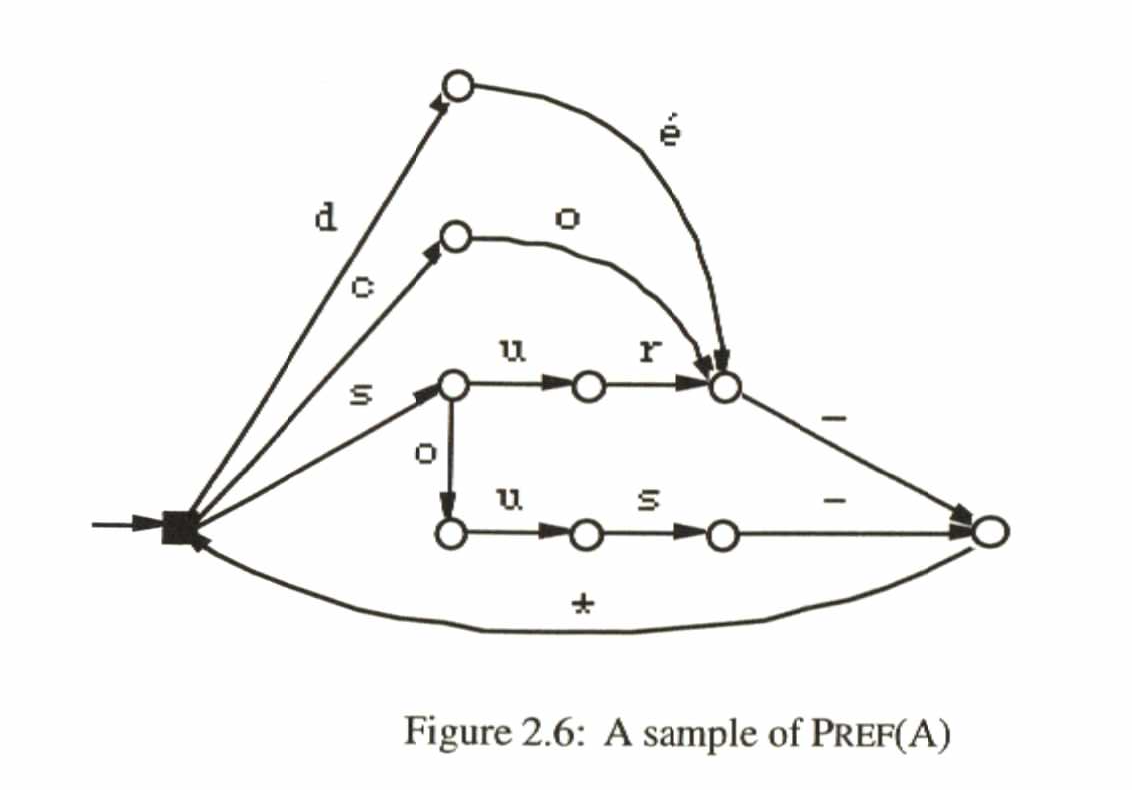
\includegraphics[width=10cm]{fig26.png}}}
  \only<2>{\centerline{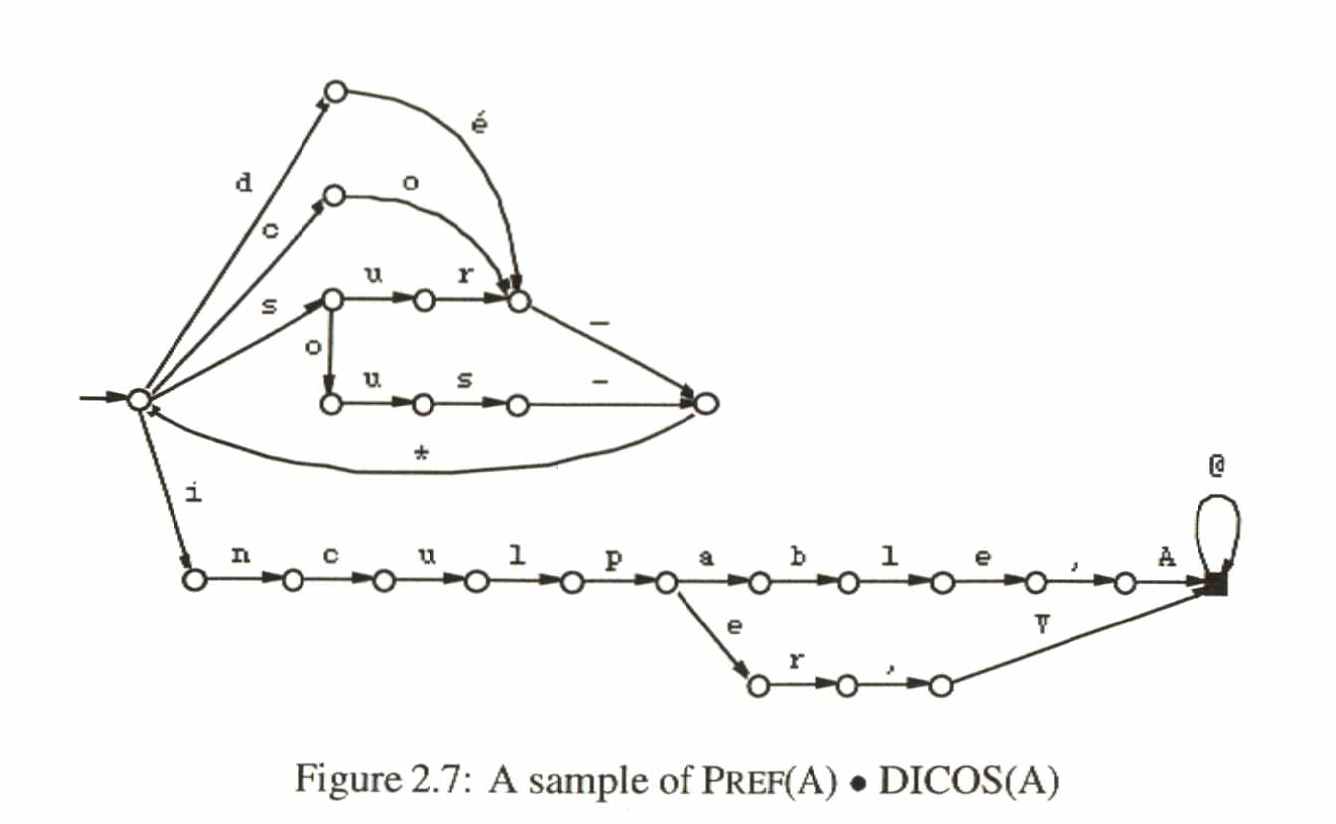
\includegraphics[width=10cm]{fig27.png}}}
  \only<3>{\centerline{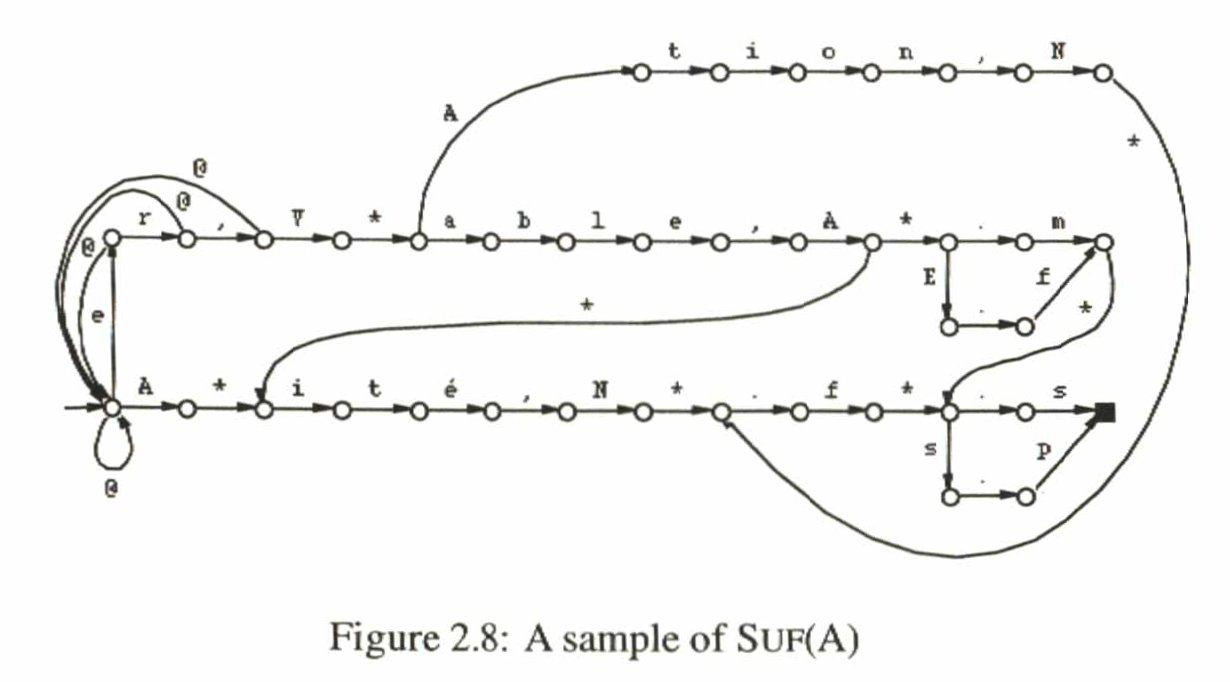
\includegraphics[width=10cm]{fig28.png}}}
  \only<4>{\centerline{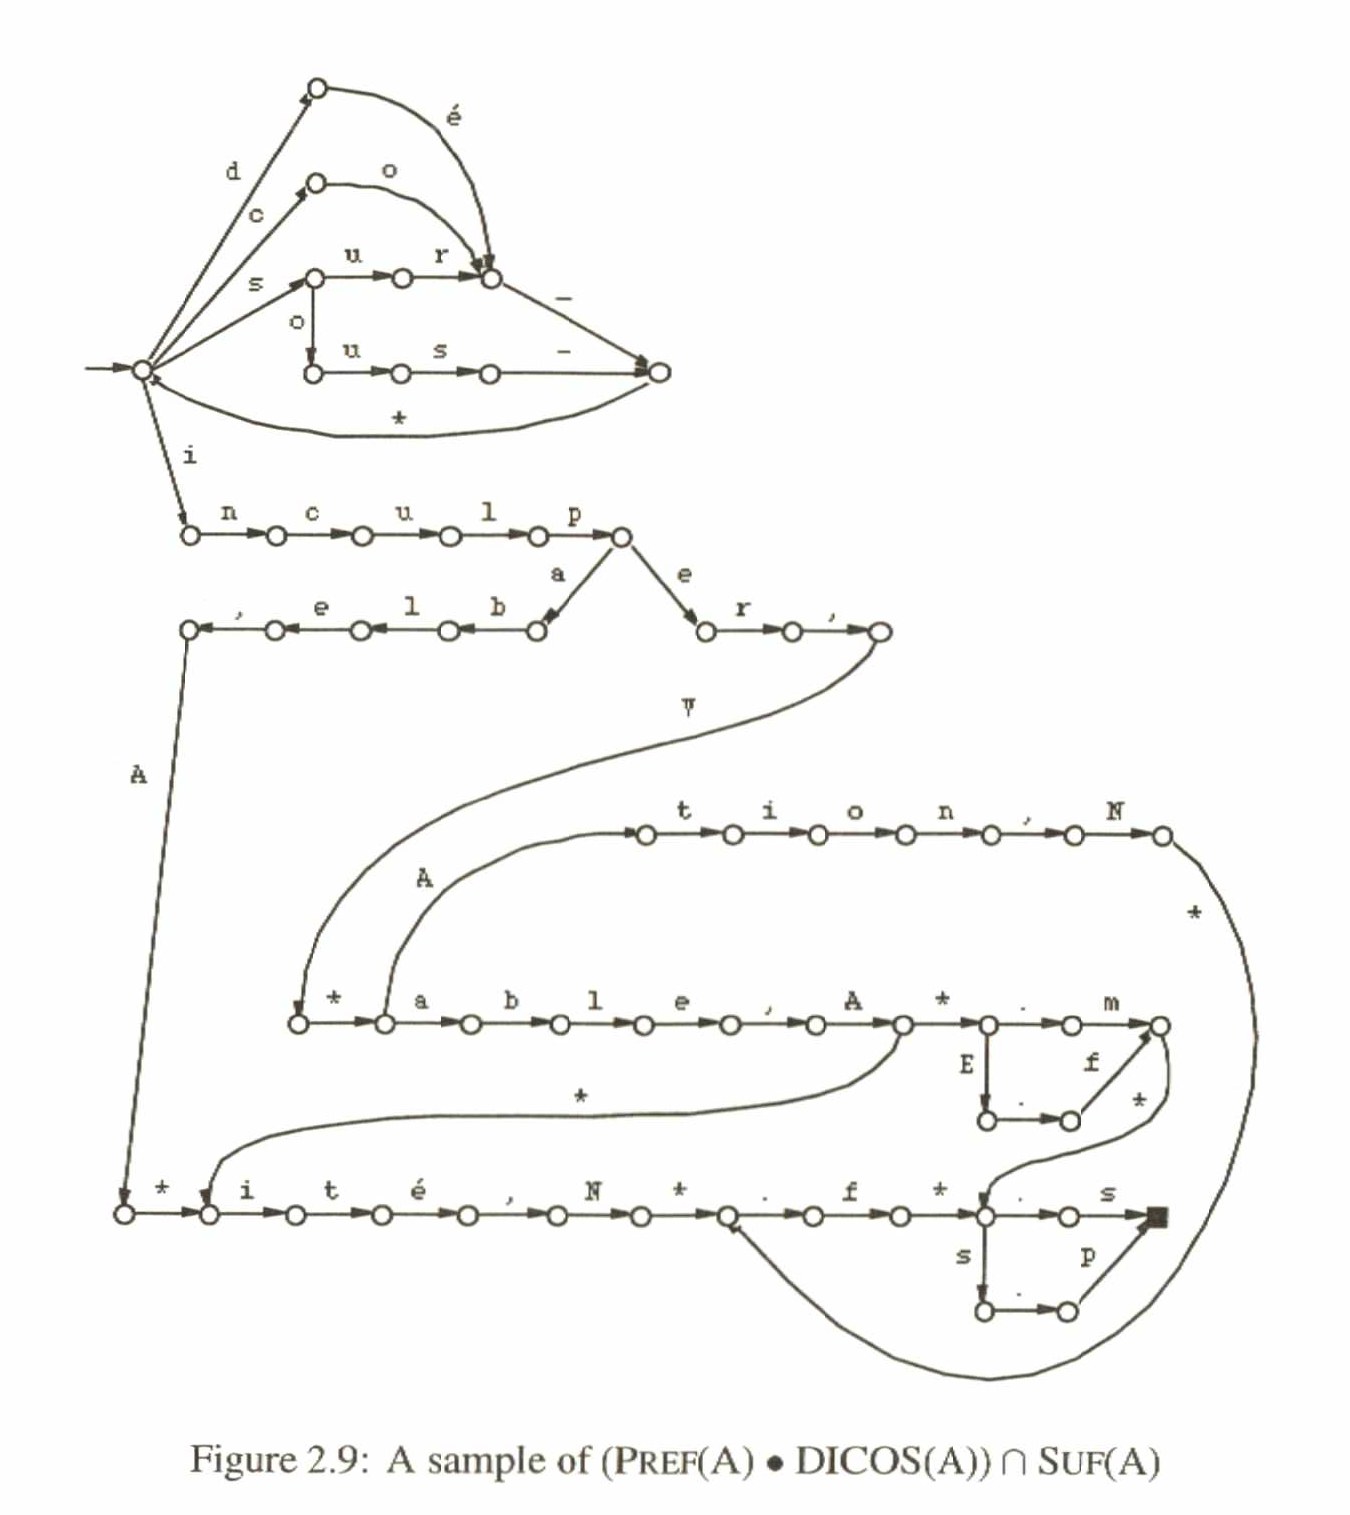
\includegraphics[height=8.5cm]{fig29.png}}}



\end{frame}

\begin{frame}[fragile]
  \frametitle{Parsing?!}
  
  CFGs are generally considered the best descriptor of natural languages

  \pause

  but they're big and slow. FSMs can help alleviate that problem. 

  \pause

  The Earley algorithm converts a deterministic CFG into a FSA by using dot notation (LR(0), LR(1)) 

  This technique involves using FSMs to model grammars by combining many grammar rules into finite states. 
\end{frame}

\begin{frame}[fragile]
  \frametitle{Advantages}

  \begin{itemize}[<+->]
    \item Compact
    \item Determinizable
    \item Symmetrical: Parsing and Production are the same process
    \item CFG $\to $ FST is a transduction\footnote{Roche 1993}
  \end{itemize}

  

  Reconceptualize parsing as a string transformation.

  \pause 

  Parser: $\Sigma_w^* \implies 2^{(\Sigma_g^* \cdot \Sigma_w^* \cdot \Sigma_g^*) }$
  
  \begingroup
  \fontsize{8pt}{12pt}\selectfont
  ``Bob left this morning'' $\iff$ ``(S(N Bob N)(V left (N this morning N)V)S)''
  \endgroup

\end{frame}

\begin{frame}[fragile]
  \frametitle{CFG}

  \centerline{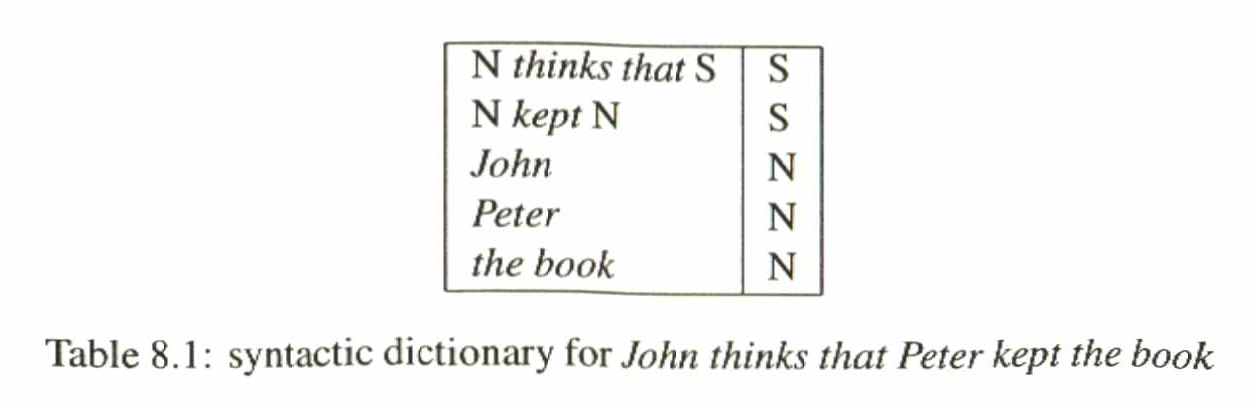
\includegraphics[width=10cm]{table81.png}}
\end{frame}

\begin{frame}[fragile]
  \frametitle{CFG}
  \centerline{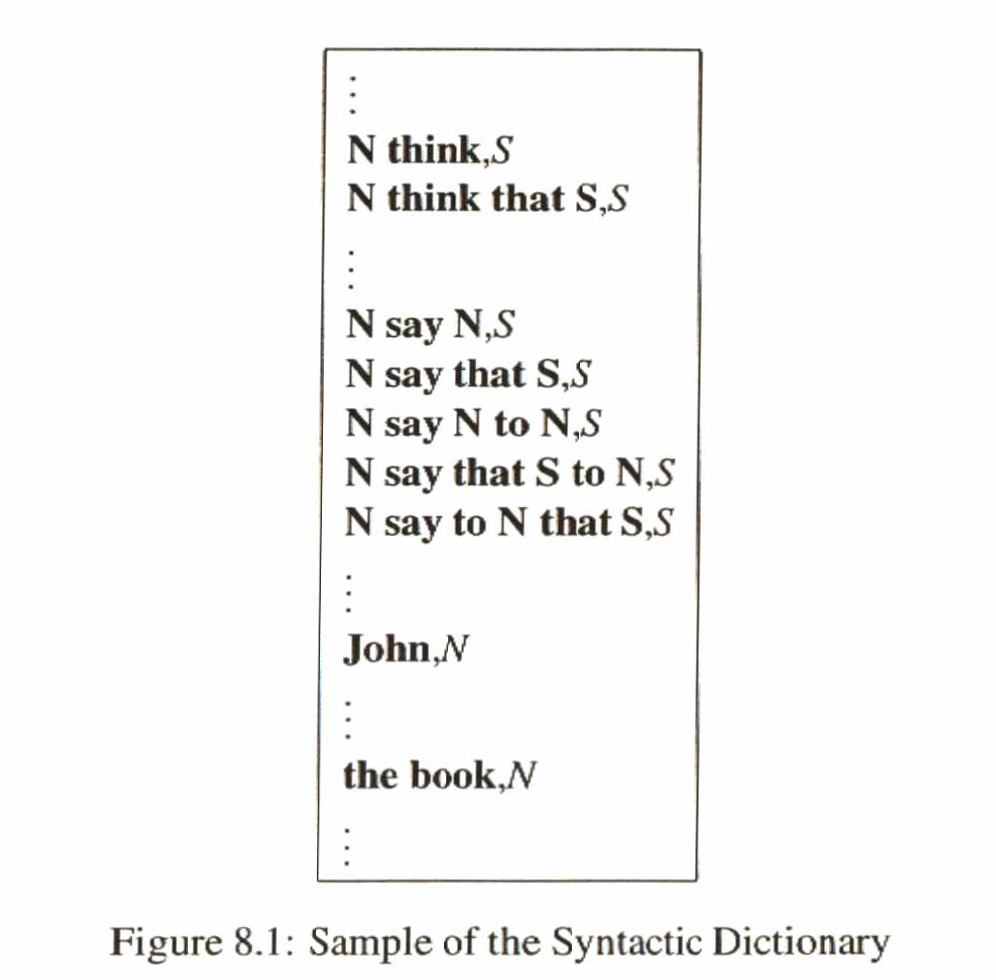
\includegraphics[height=8.5cm]{fig81.png}}  
\end{frame}

\begin{frame}[fragile]
  \frametitle{IFSP}

  \centerline{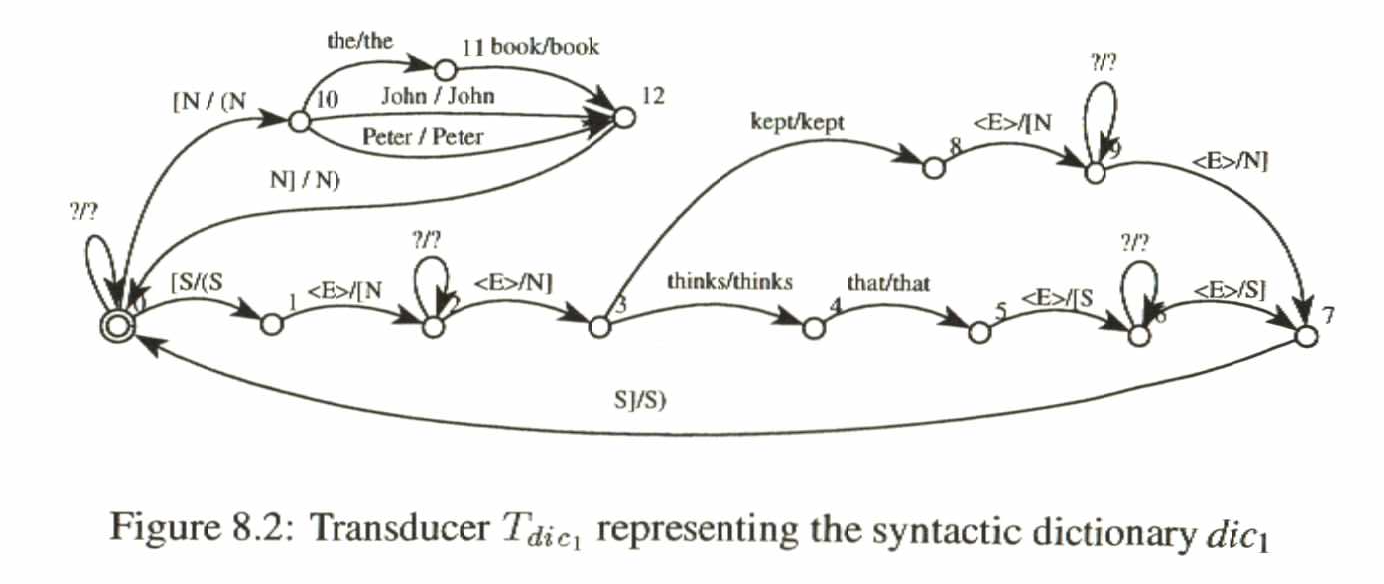
\includegraphics[width=12cm]{fig82.png}}
  
  \only<2>{[S Mike thinks that Robert kept the book S]}
  \only<3>{(S [N Mike thinks that Robert N] kept [S the book S]S)

  (S [N Mike N] thinks that [S Robert kept the book S]S)}

  \only<4>{\sout{(S [N Mike thinks that Robert N] kept [S the book S]S)}

  (S [N Mike N] thinks that [S Robert kept the book S]S)}

  \only<5>{(S (N Mike N) thinks that (S [N Robert N] kept [N the book N]S)S)}
  \only<6>{(S (N Mike N) thinks that (S (N Robert N) kept (N the book N)S)S)}

\end{frame}

\begin{frame}[fragile]
  \frametitle{Algorithm}

  \begin{lstlisting}
  TransducerParse(T, sentence):
    sent1 = sentence

    while(sent2 = Apply_Transducer(T, sent1) != sent1):
      sent1 = sent2

    return sent1

  \end{lstlisting}

  note: I haven't worked out the math, but I'm pretty sure this algorithm actually has the full power of a turing machine and can describe any Chomsky type 0 language. 
\end{frame}

\begin{frame}[fragile]
  \frametitle{Auxilliary Verb Complex}
  
  \centerline{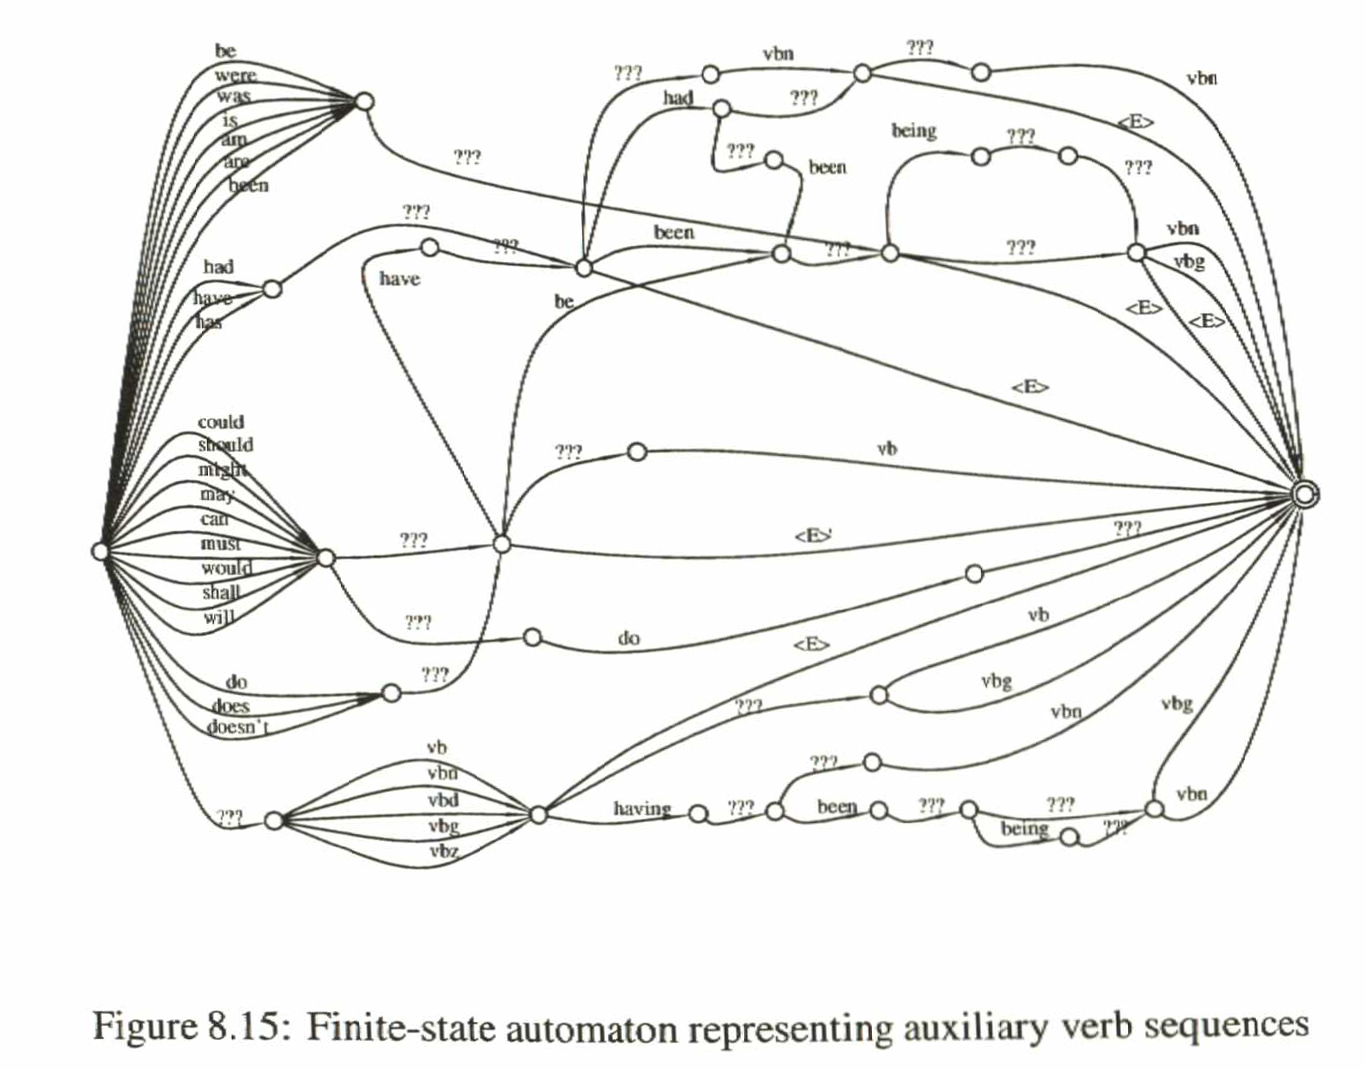
\includegraphics[width=12cm]{fig815.png}}


\end{frame}

\begin{frame}[fragile]
  \frametitle{MORE}

  \centerline{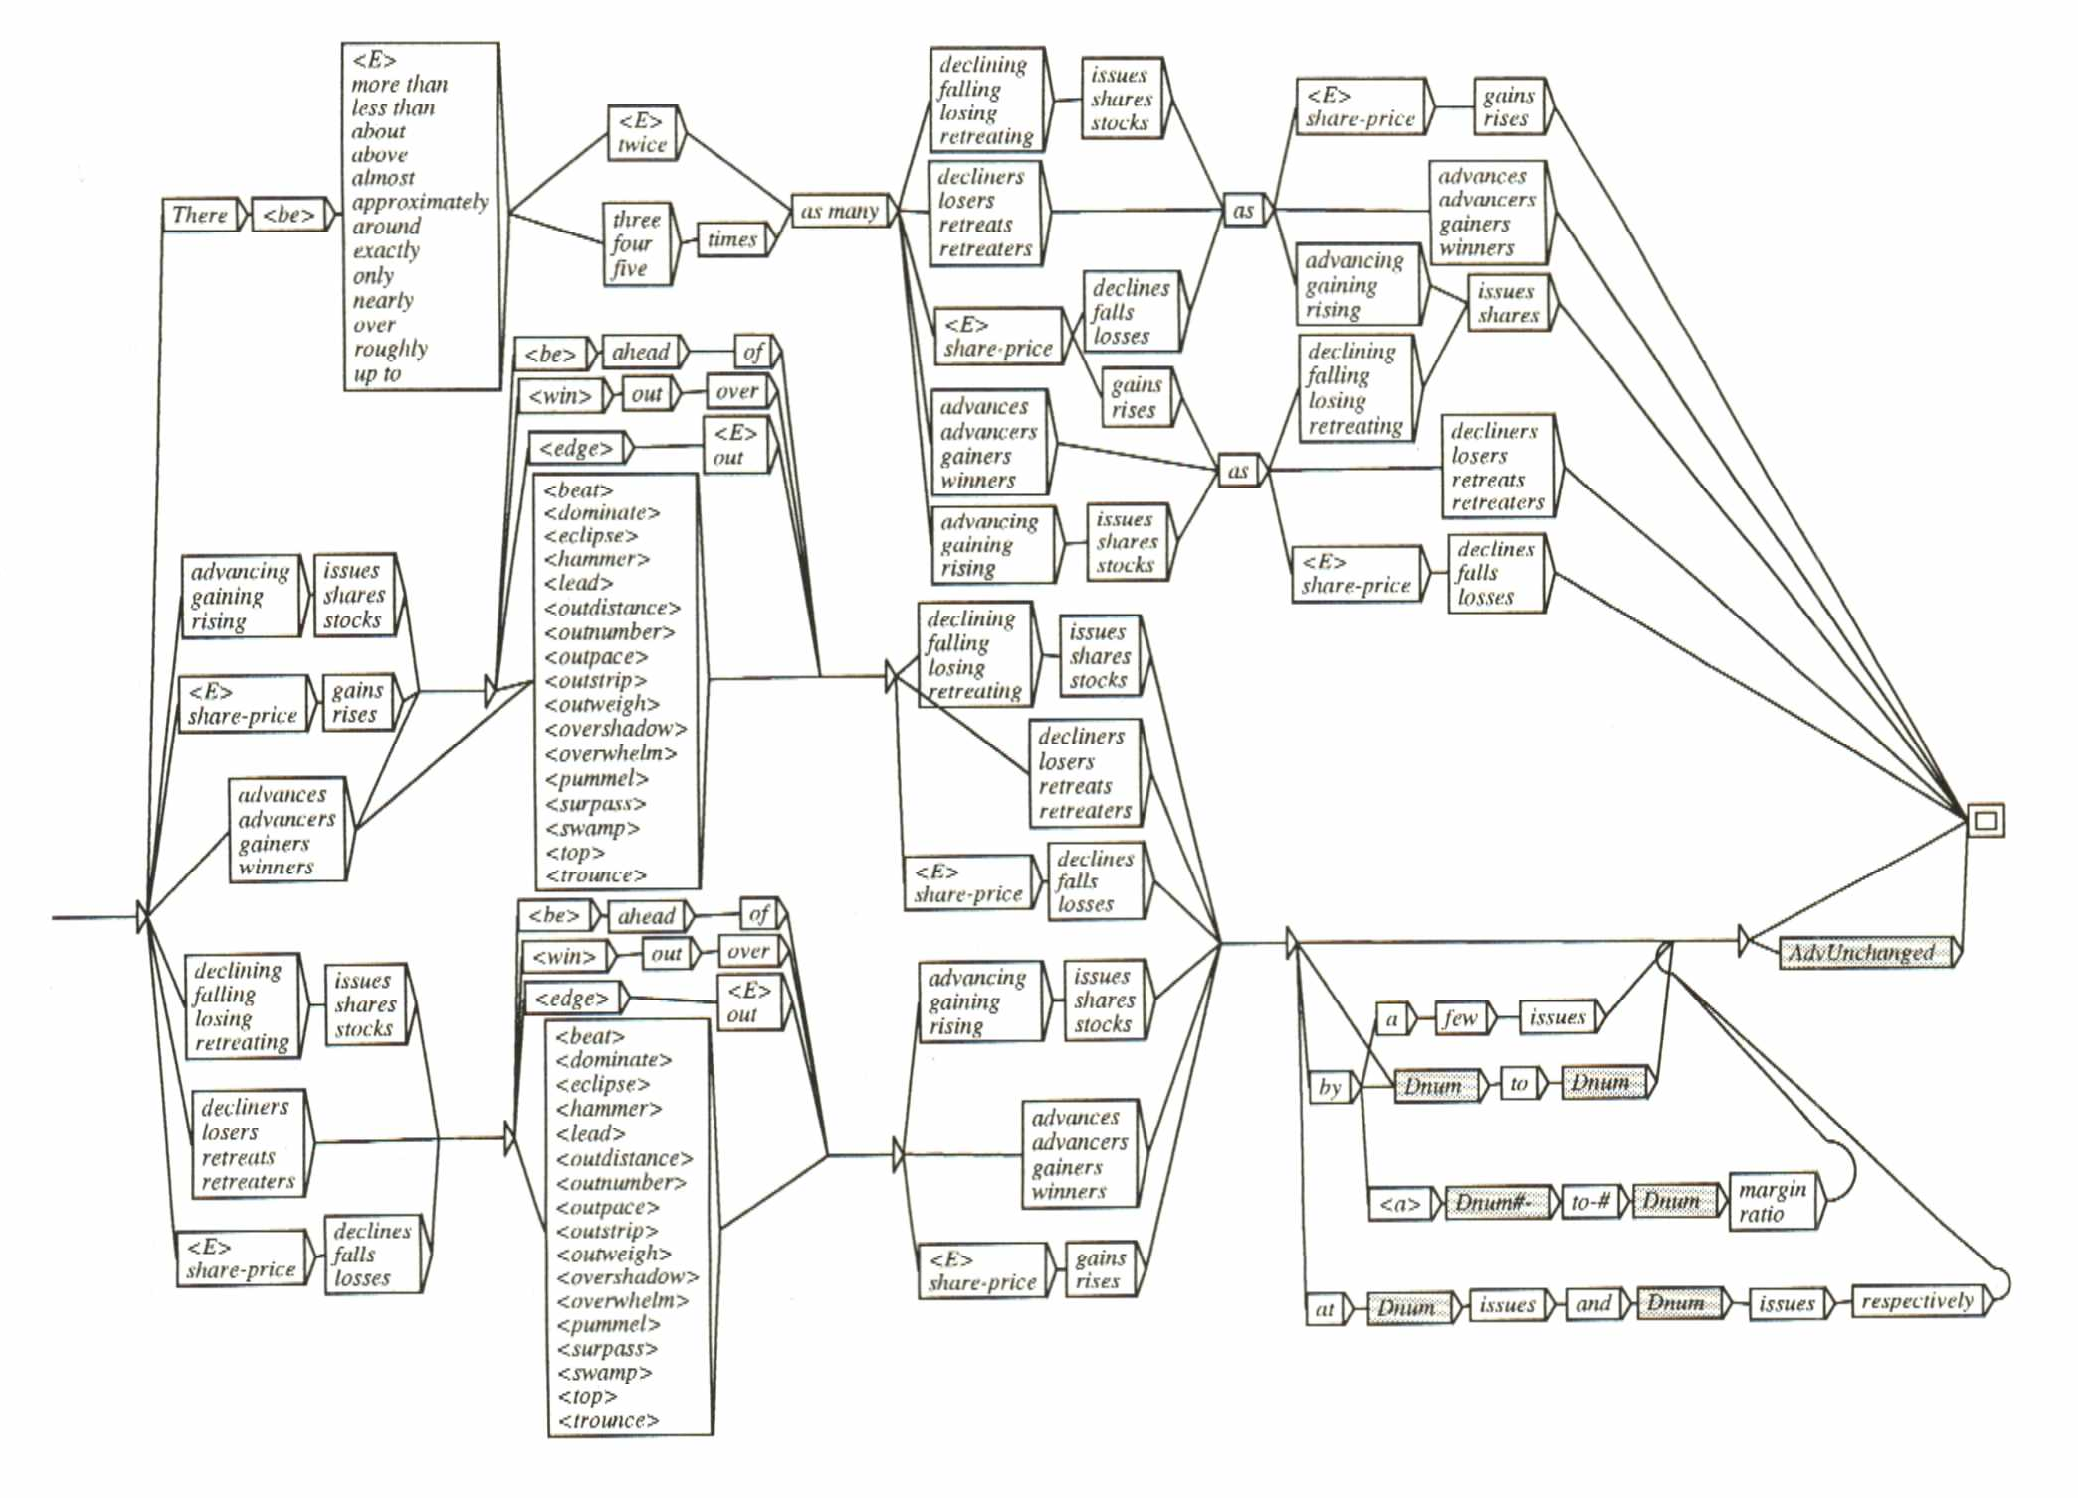
\includegraphics[width=12cm]{fig112.png}}

\end{frame}

\section*{Great, but can I use it to do real work?}



\section{Uses in NLP (search)}


\begin{frame}[fragile]
  \frametitle{Search}

  We have some data indexed with words (ie, natural language), and we want to find the correct stuff based on a query word. 

  \pause

  \textbf{How do??}  
\end{frame}

\begin{frame}[fragile]
  \frametitle{Trie}

  \pause
  \begin{columns}[T]
  \begin{column}{.48\textwidth}
  \begin{itemize}[<+->]
    \item Directed (Deteriministic)
    \item Acyclic
    \item Word
    \item Graph
  \end{itemize}
  \end{column}

  \pause
  

  \begin{column}{.48\textwidth}
  \centerline{
\includegraphics[width=6cm]{yodawg.jpg}}


  \end{column}
  \end{columns}
  

\end{frame}


\begin{frame}[fragile]
  \frametitle{Trie/DAWG}

  A finite state transducer that contains a dictionary by storing words as paths through the FSM 

\end{frame}

\begin{frame}[fragile]
  \frametitle{Trie/DAWG}
  \framesubtitle{subtitle}
  
  \centerline{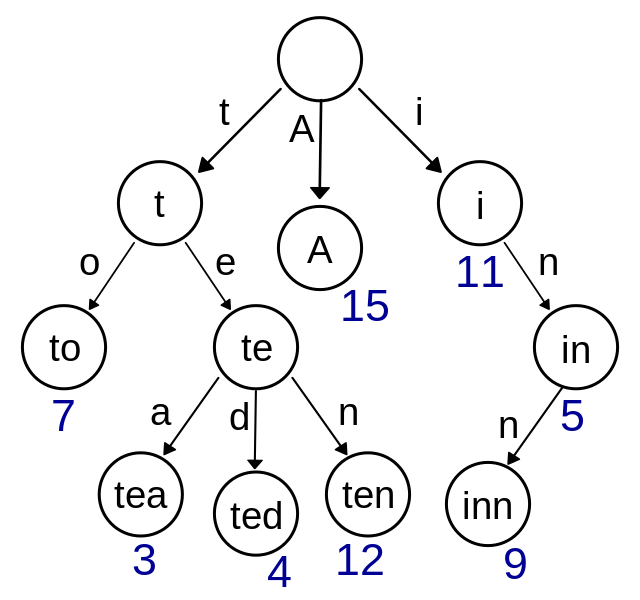
\includegraphics[height=8cm]{wikitrie.png}}
\end{frame}

\begin{frame}[fragile]
  \frametitle{Trie/DAWG}

  \begin{center}
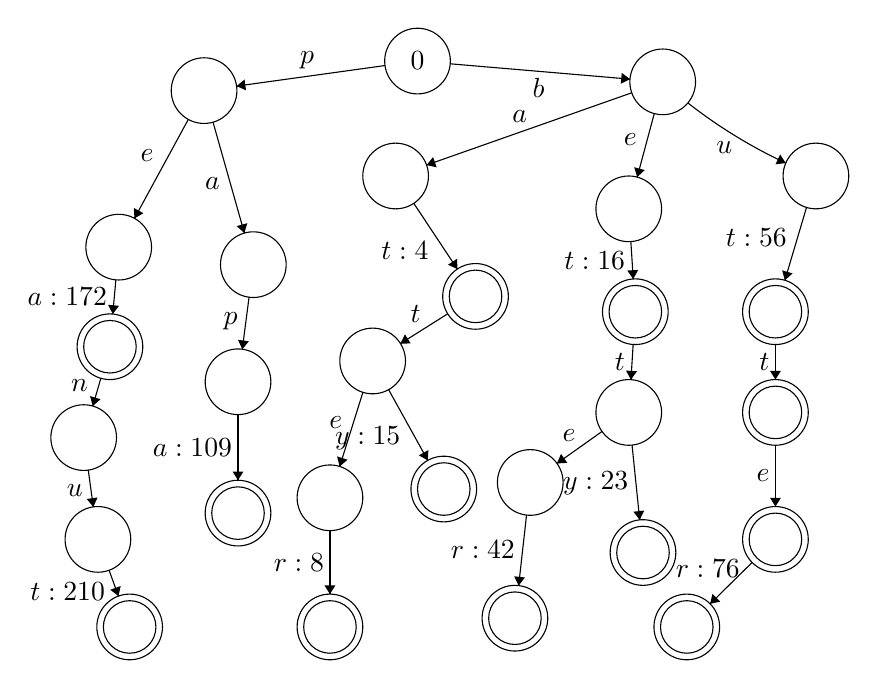
\begin{tikzpicture}[scale=0.139]
\tikzstyle{every node}+=[inner sep=0pt]
\draw [black] (38.1,-4.5) circle (3);
\draw (38.1,-4.5) node {$0$};
\draw [black] (18.6,-7.2) circle (3);
\draw [black] (10.8,-21.5) circle (3);
\draw [black] (23.1,-23.1) circle (3);
\draw [black] (10,-30.6) circle (3);
\draw [black] (10,-30.6) circle (2.4);
\draw [black] (7.6,-38.9) circle (3);
\draw [black] (8.9,-48.2) circle (3);
\draw [black] (11.8,-56.2) circle (3);
\draw [black] (11.8,-56.2) circle (2.4);
\draw [black] (21.7,-33.8) circle (3);
\draw [black] (21.7,-45.8) circle (3);
\draw [black] (21.7,-45.8) circle (2.4);
\draw [black] (60.5,-6.4) circle (3);
\draw [black] (36.1,-15) circle (3);
\draw [black] (57.4,-18) circle (3);
\draw [black] (74.5,-15) circle (3);
\draw [black] (43.4,-26) circle (3);
\draw [black] (43.4,-26) circle (2.4);
\draw [black] (34,-31.9) circle (3);
\draw [black] (40.5,-43.6) circle (3);
\draw [black] (40.5,-43.6) circle (2.4);
\draw [black] (30.1,-44.4) circle (3);
\draw [black] (30.1,-56.2) circle (3);
\draw [black] (30.1,-56.2) circle (2.4);
\draw [black] (58,-27.4) circle (3);
\draw [black] (58,-27.4) circle (2.4);
\draw [black] (57.4,-36.6) circle (3);
\draw [black] (48.4,-43) circle (3);
\draw [black] (47,-55.4) circle (3);
\draw [black] (47,-55.4) circle (2.4);
\draw [black] (58.7,-49.4) circle (3);
\draw [black] (58.7,-49.4) circle (2.4);
\draw [black] (70.8,-27.4) circle (3);
\draw [black] (70.8,-27.4) circle (2.4);
\draw [black] (70.8,-36.6) circle (3);
\draw [black] (70.8,-36.6) circle (2.4);
\draw [black] (70.8,-48.2) circle (3);
\draw [black] (70.8,-48.2) circle (2.4);
\draw [black] (62.7,-56.2) circle (3);
\draw [black] (62.7,-56.2) circle (2.4);
\draw [black] (35.13,-4.91) -- (21.57,-6.79);
\fill [black] (21.57,-6.79) -- (22.43,-7.17) -- (22.3,-6.18);
\draw (28.02,-5.26) node [above] {$p$};
\draw [black] (17.16,-9.83) -- (12.24,-18.87);
\fill [black] (12.24,-18.87) -- (13.06,-18.4) -- (12.18,-17.92);
\draw (14.03,-13.16) node [left] {$e$};
\draw [black] (19.42,-10.09) -- (22.28,-20.21);
\fill [black] (22.28,-20.21) -- (22.55,-19.31) -- (21.58,-19.58);
\draw (20.08,-15.71) node [left] {$a$};
\draw [black] (22.71,-26.07) -- (22.09,-30.83);
\fill [black] (22.09,-30.83) -- (22.69,-30.1) -- (21.7,-29.97);
\draw (21.72,-28.3) node [left] {$p$};
\draw [black] (21.7,-36.8) -- (21.7,-42.8);
\fill [black] (21.7,-42.8) -- (22.2,-42) -- (21.2,-42);
\draw (21.2,-39.8) node [left] {$a:109$};
\draw [black] (10.54,-24.49) -- (10.26,-27.61);
\fill [black] (10.26,-27.61) -- (10.83,-26.86) -- (9.83,-26.77);
\draw (9.77,-25.98) node [left] {$a:172$};
\draw [black] (9.17,-33.48) -- (8.43,-36.02);
\fill [black] (8.43,-36.02) -- (9.14,-35.39) -- (8.18,-35.11);
\draw (8.03,-34.18) node [left] {$n$};
\draw [black] (8.02,-41.87) -- (8.48,-45.23);
\fill [black] (8.48,-45.23) -- (8.87,-44.37) -- (7.88,-44.51);
\draw (7.56,-43.71) node [left] {$u$};
\draw [black] (9.92,-51.02) -- (10.78,-53.38);
\fill [black] (10.78,-53.38) -- (10.98,-52.46) -- (10.03,-52.8);
\draw (9.59,-52.98) node [left] {$t:210$};
\draw [black] (41.09,-4.75) -- (57.51,-6.15);
\fill [black] (57.51,-6.15) -- (56.76,-5.58) -- (56.67,-6.58);
\draw (49.16,-6.02) node [below] {$b$};
\draw [black] (57.67,-7.4) -- (38.93,-14);
\fill [black] (38.93,-14) -- (39.85,-14.21) -- (39.52,-13.27);
\draw (47.44,-10.17) node [above] {$a$};
\draw [black] (71.743,-13.818) arc (-115.06276:-128.06086:46.362);
\fill [black] (71.74,-13.82) -- (71.23,-13.03) -- (70.81,-13.93);
\draw (66.12,-11.83) node [below] {$u$};
\draw [black] (59.73,-9.3) -- (58.17,-15.1);
\fill [black] (58.17,-15.1) -- (58.86,-14.46) -- (57.9,-14.2);
\draw (58.19,-11.69) node [left] {$e$};
\draw [black] (37.76,-17.5) -- (41.74,-23.5);
\fill [black] (41.74,-23.5) -- (41.72,-22.56) -- (40.88,-23.11);
\draw (39.14,-21.83) node [left] {$t:4$};
\draw [black] (40.86,-27.59) -- (36.54,-30.31);
\fill [black] (36.54,-30.31) -- (37.48,-30.3) -- (36.95,-29.46);
\draw (37.92,-28.45) node [above] {$t$};
\draw [black] (33.11,-34.76) -- (30.99,-41.54);
\fill [black] (30.99,-41.54) -- (31.71,-40.92) -- (30.75,-40.62);
\draw (31.28,-37.51) node [left] {$e$};
\draw [black] (30.1,-47.4) -- (30.1,-53.2);
\fill [black] (30.1,-53.2) -- (30.6,-52.4) -- (29.6,-52.4);
\draw (29.6,-50.3) node [left] {$r:8$};
\draw [black] (35.46,-34.52) -- (39.04,-40.98);
\fill [black] (39.04,-40.98) -- (39.09,-40.04) -- (38.22,-40.52);
\draw (36.58,-38.95) node [left] {$y:15$};
\draw [black] (57.59,-20.99) -- (57.81,-24.41);
\fill [black] (57.81,-24.41) -- (58.26,-23.58) -- (57.26,-23.64);
\draw (57.11,-22.74) node [left] {$t:16$};
\draw [black] (57.8,-30.39) -- (57.6,-33.61);
\fill [black] (57.6,-33.61) -- (58.15,-32.84) -- (57.15,-32.78);
\draw (57.1,-31.96) node [left] {$t$};
\draw [black] (57.7,-39.58) -- (58.4,-46.42);
\fill [black] (58.4,-46.42) -- (58.81,-45.57) -- (57.82,-45.67);
\draw (57.41,-43.09) node [left] {$y:23$};
\draw [black] (54.96,-38.34) -- (50.84,-41.26);
\fill [black] (50.84,-41.26) -- (51.79,-41.21) -- (51.21,-40.39);
\draw (51.95,-39.3) node [above] {$e$};
\draw [black] (48.06,-45.98) -- (47.34,-52.42);
\fill [black] (47.34,-52.42) -- (47.92,-51.68) -- (46.93,-51.57);
\draw (47.04,-49.09) node [left] {$r:42$};
\draw [black] (73.64,-17.87) -- (71.66,-24.53);
\fill [black] (71.66,-24.53) -- (72.37,-23.9) -- (71.41,-23.62);
\draw (71.88,-20.6) node [left] {$t:56$};
\draw [black] (70.8,-30.4) -- (70.8,-33.6);
\fill [black] (70.8,-33.6) -- (71.3,-32.8) -- (70.3,-32.8);
\draw (70.3,-32) node [left] {$t$};
\draw [black] (70.8,-39.6) -- (70.8,-45.2);
\fill [black] (70.8,-45.2) -- (71.3,-44.4) -- (70.3,-44.4);
\draw (70.3,-42.4) node [left] {$e$};
\draw [black] (68.67,-50.31) -- (64.83,-54.09);
\fill [black] (64.83,-54.09) -- (65.75,-53.89) -- (65.05,-53.17);
\draw (64.62,-51.72) node [above] {$r:76$};
\end{tikzpicture}
\end{center}

\end{frame}


\begin{frame}[c]
  \frametitle{Cool, so what?}

  \pause

  \centering
  If only there was a way to take steps through the trie that are close to but not exactly the same as the query...

\end{frame}

\begin{frame}[fragile]
  \frametitle{Levenshtein}

  \pause

  \centering
\begin{tabular}{ r || c c c c c c  }
  r &   &  &  &  &  &  \\
  e &   &  &  &  &  &  \\
  t &   &  &  &  &  &  \\ 
  t &   &  &  &  &  &  \\
  u &   &  &  &  &  &  \\
  B &   &  &  &  &  &  \\
    & 0 &  &  &  &  &  \\
  \hline
    &   & B & e & t & t & r \\
\end{tabular}

  
\end{frame}

\begin{frame}[fragile]
  \frametitle{Levenshtein}

  \centering
\begin{tabular}{ r || c c c c c c  }
  r &   &  &  &  &  &  \\
  e &   &  &  &  &  &  \\
  t &   &  &  &  &  &  \\ 
  t &   &  &  &  &  &  \\
  u &   &  &  &  &  &  \\
  B & 1 &  &  &  &  &  \\
    & 0 &  &  &  &  &  \\
  \hline
    &   & B & e & t & t & r \\
\end{tabular}

  
\end{frame}



\begin{frame}[fragile]
  \frametitle{Levenshtein}

  \centering
\begin{tabular}{ r || c c c c c c  }
  r &   &  &  &  &  &  \\
  e &   &  &  &  &  &  \\
  t &   &  &  &  &  &  \\ 
  t &   &  &  &  &  &  \\
  u & 2 &  &  &  &  &  \\
  B & 1 &  &  &  &  &  \\
    & 0 &  &  &  &  &  \\
  \hline
    &   & B & e & t & t & r \\
\end{tabular}

  
\end{frame}


\begin{frame}[fragile]
  \frametitle{Levenshtein}

  \centering
\begin{tabular}{ r || c c c c c c  }
  r & 6 &  &  &  &  &  \\
  e & 5 &  &  &  &  &  \\
  t & 4 &  &  &  &  &  \\
  t & 3 &  &  &  &  &  \\
  u & 2 &  &  &  &  &  \\
  B & 1 &  &  &  &  &  \\
    & 0 &  &  &  &  &  \\
  \hline
    &   & B & e & t & t & r \\
\end{tabular}

  
\end{frame}

\begin{frame}[fragile]
  \frametitle{Levenshtein}

  \centering
\begin{tabular}{ r || c c c c c c  }
  r & 6 & 5 &  &  &  &  \\
  e & 5 & 4 &  &  &  &  \\
  t & 4 & 3 &  &  &  &  \\
  t & 3 & 2 &  &  &  &  \\
  u & 2 & 1 &  &  &  &  \\
  B & 1 & 0 &  &  &  &  \\
    & 0 & 1 &  &  &  &  \\
  \hline
    &   & B & e & t & t & r \\
\end{tabular}

  
\end{frame}

\begin{frame}[fragile]
  \frametitle{Levenshtein}

  \centering
\begin{tabular}{ r || c c c c c c  }
  r & 6 & 5 & 4 &  &  &  \\
  e & 5 & 4 & 3 &  &  &  \\
  t & 4 & 3 & 3 &  &  &  \\
  t & 3 & 2 & 2 &  &  &  \\
  u & 2 & 1 & 1 &  &  &  \\
  B & 1 & 0 & 1 &  &  &  \\
    & 0 & 1 & 2 &  &  &  \\
  \hline
    &   & B & e & t & t & r \\
\end{tabular}

  
\end{frame}


\begin{frame}[fragile]
  \frametitle{Levenshtein}

  \centering
\begin{tabular}{ r || c c c c c c  }
  r & 6 & 5 & 4 & 3 &  &  \\
  e & 5 & 4 & 3 & 2 &  &  \\
  t & 4 & 3 & 3 & 1 &  &  \\
  t & 3 & 2 & 2 & 1 &  &  \\
  u & 2 & 1 & 1 & 2 &  &  \\
  B & 1 & 0 & 1 & 2 &  &  \\
    & 0 & 1 & 2 & 3 &  &  \\
  \hline
    &   & B & e & t & t & r \\
\end{tabular}

  
\end{frame}

\begin{frame}[fragile]
  \frametitle{Levenshtein}

  \centering
\begin{tabular}{ r || c c c c c c  }
  r & 6 & 5 & 4 & 3 & 3 &  \\
  e & 5 & 4 & 3 & 2 & 2 &  \\
  t & 4 & 3 & 3 & 1 & 1 &  \\
  t & 3 & 2 & 2 & 1 & 1 &  \\
  u & 2 & 1 & 1 & 2 & 3 &  \\
  B & 1 & 0 & 1 & 2 & 3 &  \\
    & 0 & 1 & 2 & 3 & 4 &  \\
  \hline
    &   & B & e & t & t & r \\
\end{tabular}

  
\end{frame}



\begin{frame}[fragile]
  \frametitle{Levenshtein}

  \centering
\begin{tabular}{ r || c c c c c c  }
  r & 6 & 5 & 4 & 3 & 3 & 2 \\
  e & 5 & 4 & 3 & 2 & 2 & 2 \\
  t & 4 & 3 & 3 & 1 & 1 & 2 \\
  t & 3 & 2 & 2 & 1 & 1 & 2 \\
  u & 2 & 1 & 1 & 2 & 3 & 4 \\
  B & 1 & 0 & 1 & 2 & 3 & 4 \\
    & 0 & 1 & 2 & 3 & 4 & 5 \\
  \hline
    &   & B & e & t & t & r \\
\end{tabular}

  Levenshtein distance: 2
  \pause

  Way too expensive to do for every string
  \pause

   but...
\end{frame}























\begin{frame}[fragile]
  \frametitle{Levenshtein Automata}

  \pause

  \centering
\begin{tabular}{ r || c | c | c | c | c | c  }
  r & 6 & 5 & 4 & 3 & 3 & 2 \\
  e & 5 & 4 & 3 & 2 & 2 & 2 \\
  t & 4 & 3 & 3 & 1 & 1 & 2 \\ 
  t & 3 & 2 & 2 & 1 & 1 & 2 \\
  u & 2 & 1 & 1 & 2 & 3 & 4 \\
  B & 1 & 0 & 1 & 2 & 3 & 4 \\
    & 0 & 1 & 2 & 3 & 4 & 5 \\
  \hline
    &   & B & e & t & t & r \\
\end{tabular}

  Mihov and Schultz (2002)
\end{frame}


\begin{frame}[fragile]
  \frametitle{Python implementation}

  \begingroup
  \fontsize{8pt}{10pt}\selectfont
  \begin{lstlisting}[language=python]
  class LevenshteinAutomaton:
    def __init__(self, string, n):
        self.string = string
        self.max_edits = n
    def start(self):
        return range(len(self.string)+1)
    def step(self, state, c):
        new_state = [state[0]+1]
        for i in range(len(state)-1):
            cost = 0 if self.string[i] == c else 1
            new_state.append(min(new_state[i]+1, state[i]+cost, 
              state[i+1]+1))
        return [min(x,self.max_edits+1) for x in new_state]
    def is_match(self, state):
        return state[-1] <= self.max_edits
    def can_match(self, state):
        return min(state) <= self.max_edits



  \end{lstlisting}  
  \endgroup
\end{frame}

\begin{frame}[fragile]
  \frametitle{Levenshtein Automaton (credit to Jules Jacobs)}


  \centerline{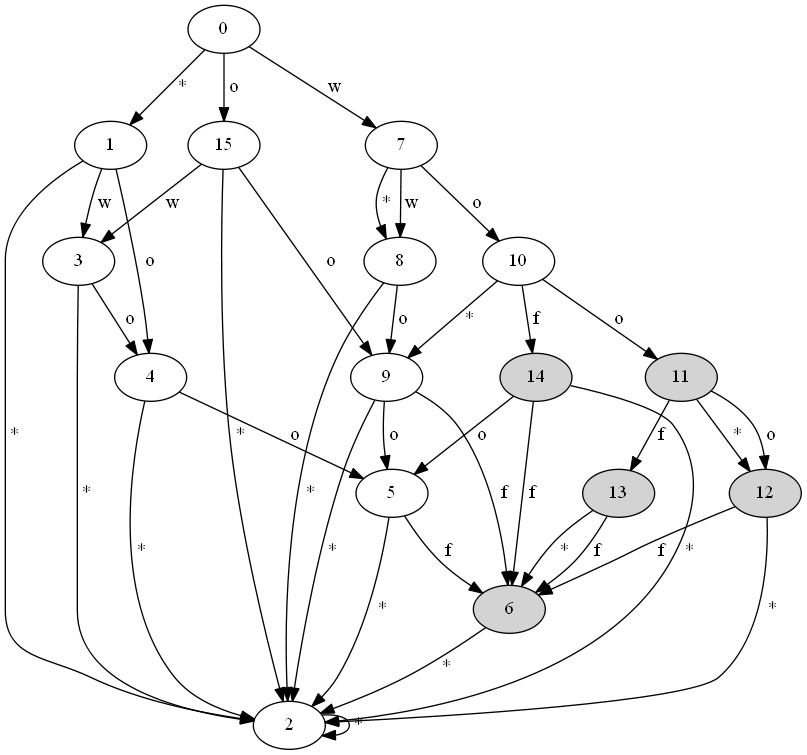
\includegraphics[height=8cm]{levautomaton.png}}  
\end{frame}

\begin{frame}[fragile]
  \frametitle{Properties}
  \pause

  Numbers of states is linearly bounded by the length of the query string

  \pause

  builds in O(n) time

  \pause

  (can cut that down to O($\delta$) by using sparse vectors)
\end{frame}

\begin{frame}[fragile]
  \frametitle{Use}

  \begin{figure}
  \centering
  \begin{subfigure}
  \centering
    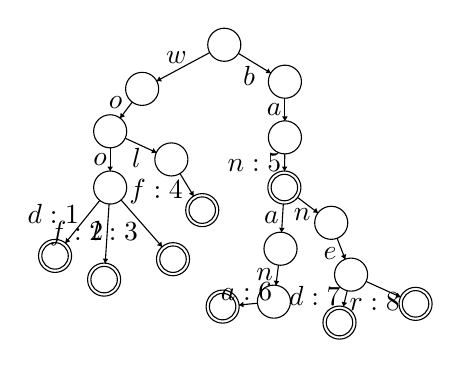
\begin{tikzpicture}[scale=0.07]
    \tikzstyle{every node}+=[inner sep=0pt]
    \draw [black] (39.5,-6.7) circle (3);
    \draw [black] (24.6,-14.7) circle (3);
    \draw [black] (18.8,-22.4) circle (3);
    \draw [black] (18.8,-32.6) circle (3);
    \draw [black] (17.7,-49.3) circle (3);
    \draw [black] (17.7,-49.3) circle (2.4);
    \draw [black] (8.8,-45) circle (3);
    \draw [black] (8.8,-45) circle (2.4);
    \draw [black] (50.5,-13.4) circle (3);
    \draw [black] (50.5,-23.5) circle (3);
    \draw [black] (50.4,-32.6) circle (3);
    \draw [black] (50.4,-32.6) circle (2.4);
    \draw [black] (49.7,-43.7) circle (3);
    \draw [black] (48.5,-53.3) circle (3);
    \draw [black] (39.2,-54.2) circle (3);
    \draw [black] (39.2,-54.2) circle (2.4);
    \draw [black] (58.9,-39) circle (3);
    \draw [black] (62.5,-48.4) circle (3);
    \draw [black] (60.4,-57.1) circle (3);
    \draw [black] (60.4,-57.1) circle (2.4);
    \draw [black] (74.2,-53.7) circle (3);
    \draw [black] (74.2,-53.7) circle (2.4);
    \draw [black] (30.2,-45.6) circle (3);
    \draw [black] (30.2,-45.6) circle (2.4);
    \draw [black] (29.9,-27.5) circle (3);
    \draw [black] (35.5,-36.7) circle (3);
    \draw [black] (35.5,-36.7) circle (2.4);
    \draw [black] (36.86,-8.12) -- (27.24,-13.28);
    \fill [black] (27.24,-13.28) -- (28.18,-13.34) -- (27.71,-12.46);
    \draw (30.83,-10.2) node [above] {$w$};
    \draw [black] (22.8,-17.1) -- (20.6,-20);
    \fill [black] (20.6,-20) -- (21.49,-19.67) -- (20.69,-19.06);
    \draw (21.12,-17.15) node [left] {$o$};
    \draw [black] (18.8,-25.4) -- (18.8,-29.6);
    \fill [black] (18.8,-29.6) -- (19.3,-28.8) -- (18.3,-28.8);
    \draw (18.3,-27.5) node [left] {$o$};
    \draw [black] (18.6,-35.59) -- (17.9,-46.31);
    \fill [black] (17.9,-46.31) -- (18.45,-45.54) -- (17.45,-45.48);
    \draw (17.65,-40.91) node [left] {$f:2$};
    \draw [black] (16.92,-34.94) -- (10.68,-42.66);
    \fill [black] (10.68,-42.66) -- (11.57,-42.36) -- (10.8,-41.73);
    \draw (13.24,-37.37) node [left] {$d:1$};
    \draw [black] (20.78,-34.86) -- (28.22,-43.34);
    \fill [black] (28.22,-43.34) -- (28.07,-42.41) -- (27.32,-43.07);
    \draw (23.96,-40.55) node [left] {$l:3$};
    \draw [black] (42.06,-8.26) -- (47.94,-11.84);
    \fill [black] (47.94,-11.84) -- (47.51,-11) -- (46.99,-11.85);
    \draw (44,-10.55) node [below] {$b$};
    \draw [black] (50.5,-16.4) -- (50.5,-20.5);
    \fill [black] (50.5,-20.5) -- (51,-19.7) -- (50,-19.7);
    \draw (50,-18.45) node [left] {$a$};
    \draw [black] (50.47,-26.5) -- (50.43,-29.6);
    \fill [black] (50.43,-29.6) -- (50.94,-28.81) -- (49.94,-28.79);
    \draw (49.93,-28.05) node [left] {$n:5$};
    \draw [black] (52.8,-34.4) -- (56.5,-37.2);
    \fill [black] (56.5,-37.2) -- (56.17,-36.31) -- (55.56,-37.11);
    \draw (53.65,-36.3) node [below] {$n$};
    \draw [black] (59.97,-41.8) -- (61.43,-45.6);
    \fill [black] (61.43,-45.6) -- (61.61,-44.67) -- (60.67,-45.03);
    \draw (59.95,-44.54) node [left] {$e$};
    \draw [black] (61.8,-51.32) -- (61.1,-54.18);
    \fill [black] (61.1,-54.18) -- (61.78,-53.52) -- (60.81,-53.29);
    \draw (60.69,-52.32) node [left] {$d:7$};
    \draw [black] (65.23,-49.64) -- (71.47,-52.46);
    \fill [black] (71.47,-52.46) -- (70.94,-51.68) -- (70.53,-52.59);
    \draw (66.77,-51.56) node [below] {$r:8$};
    \draw [black] (50.21,-35.59) -- (49.89,-40.71);
    \fill [black] (49.89,-40.71) -- (50.44,-39.94) -- (49.44,-39.88);
    \draw (49.46,-38.11) node [left] {$a$};
    \draw [black] (49.33,-46.68) -- (48.87,-50.32);
    \fill [black] (48.87,-50.32) -- (49.47,-49.59) -- (48.48,-49.47);
    \draw (48.43,-48.37) node [left] {$n$};
    \draw [black] (45.51,-53.59) -- (42.19,-53.91);
    \fill [black] (42.19,-53.91) -- (43.03,-54.33) -- (42.93,-53.34);
    \draw (43.54,-53.11) node [above] {$a:6$};
    \draw [black] (21.53,-23.65) -- (27.17,-26.25);
    \fill [black] (27.17,-26.25) -- (26.66,-25.46) -- (26.24,-26.37);
    \draw (23.59,-25.46) node [below] {$l$};
    \draw [black] (31.46,-30.06) -- (33.94,-34.14);
    \fill [black] (33.94,-34.14) -- (33.95,-33.19) -- (33.1,-33.71);
    \draw (32.06,-33.37) node [left] {$f:4$};
    \end{tikzpicture}
  \end{subfigure}
  \pause
  \begin{subfigure}
  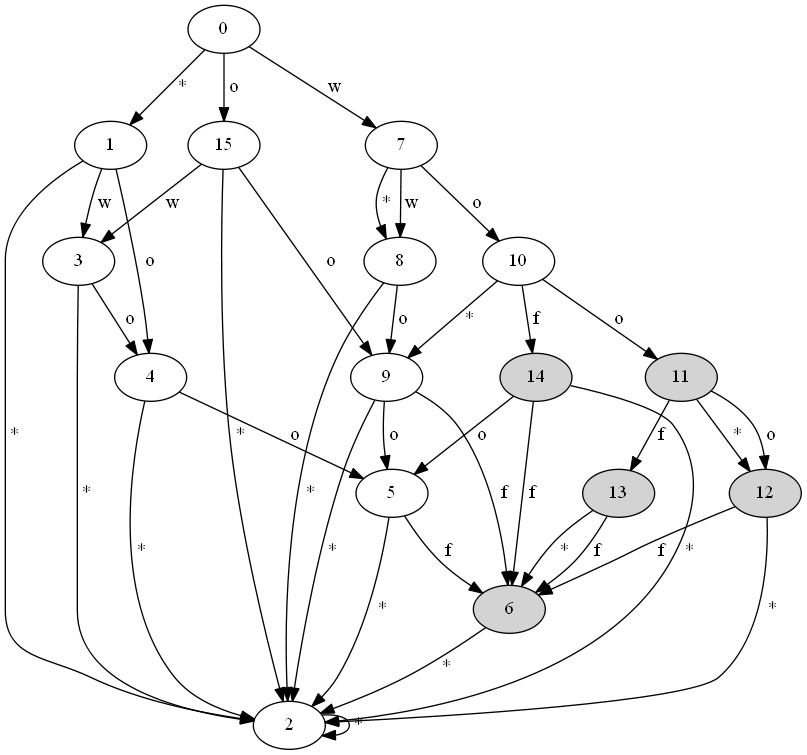
\includegraphics[width=5cm]{levautomaton.png}

  \end{subfigure}
  \end{figure}
  
\end{frame}







\section{Wrap-up}

\begin{frame}{Summary}

  We can do better. 

  \pause

  What if we don't have the whole search term from the user to make a Levenshtein Automaton with? 

  \pause

  What if it's only a prefix?

  \pause

  There still isn't a super efficient way to do fuzzy prefix searching.
\end{frame}

\begin{frame}[standout]
  Questions?
\end{frame}

\appendix

\begin{frame}[t]
  \frametitle{Tools and resources}
  
  \begin{description}
    \item[Apache Lucene] full stack FOSS search solution

    \item[Marisa\_trie] Python trie, shares interface with DAWG

    \item[DAWG] another Python trie

    \item[Roche and Schabes 1997] primary source on FS comp ling

    \item[Mihov and Schultz 2002] levenshtein automata
  \end{description}
  
\end{frame}




\begin{frame}[allowframebreaks]{References}

  \nocite{*}
  \bibliography{trevor-minimalist-machine}
  \bibliographystyle{abbrv}

\end{frame}

\end{document}
